\documentclass{experimentreport}

\usepackage{listings}
\usepackage{xcolor}

\definecolor{codegreen}{rgb}{0,0.6,0}
\definecolor{codegray}{rgb}{0.5,0.5,0.5}
\definecolor{codepurple}{rgb}{0.58,0,0.82}
\definecolor{backcolour}{rgb}{0.95,0.95,0.92}
\definecolor{lightgreen}{rgb}{0,0.4,0}
\definecolor{lightred}{rgb}{0.4,0,0}

\definecolor{mygray}{gray}{.9}

% \lstdefinestyle{mystyle}{
\lstset{
    %backgroundcolor=\color{backcolour},   
    commentstyle=\color{brown},
    keywordstyle=\color{magenta},
    numberstyle=\tiny\color{codegray},
    stringstyle=\color{codepurple},
    basicstyle=\ttfamily\tiny,
    breakatwhitespace=false,         
    breaklines=true,                 
    captionpos=b,                    
    keepspaces=true,                 
    numbers=none,                    
    numbersep=5pt,                  
    showspaces=false,                
    showstringspaces=false,
    showtabs=false,                  
    tabsize=2,
    escapeinside={<@}{@>}
}

% \lstset{
% basicstyle=\ttfamily\bfseries\footnotesize,
%   morekeywords={virtualinvoke},
%   keywordstyle=,
%   ndkeywordstyle=\color{red},
%   commentstyle=\color{gray},
%   stringstyle=\color{green},
%   numbers=none,
%   breaklines=true,
%   numberstyle=\ttfamily\footnotesize\color{gray},
%   stepnumber=1,
%   numbersep=6pt,
%   backgroundcolor=\color{white},
%   tabsize=4,
%   showspaces=false,
%   showstringspaces=false,
%   xleftmargin=6pt,
%   captionpos=t
% }

\lstdefinelanguage{JavaScript}{
  keywords={typeof, new, true, false, catch, function, return, null, catch, switch, var, if, in, while, do, else, case, break, export, static, const, let, class, void, async, await, interface, extends, public, this},
  % basicstyle=\linespread{1.0}\ttfamily\footnotesize,
  % keywordstyle= \color{violet}\bfseries,
  ndkeywords={class, export, boolean, throw, implements, import, this},
  ndkeywordstyle=\color{darkgray}\bfseries,
  identifierstyle=\color{black},
  sensitive=false,
  frame=lines,
  comment=[l]{//},
  morecomment=[s]{/*}{*/},
  % commentstyle=\color{gray}\ttfamily,
  % stringstyle=\color{blue}\ttfamily,
  morestring=[b]',
  morestring=[b]"
}



\usepackage{graphicx}
\usepackage{hyperref}
\usepackage{enumitem}
\usepackage{amsmath}
\usepackage{booktabs}
\usepackage{multirow}
\usepackage{xcolor}
\usepackage{colortbl}
% 新增 caption 宏包以解决宏包内浮动体的问题
\usepackage{caption}

%========================
% 基本信息
%========================

\setcoursename{基础软件开发技术实践}
\setreportname{智能软件工程实验报告}

\setexperimenttitle{实验三：基于大语言模型的人类编写代码的代码审查}

\setstudentname{\hintholder{廖正强}}
\setdepartment{\hintholder{计算学部}}
\setstudentid{\hintholder{2023112920}}

\setcourseteacher{刘佳琨}
\setinstructor{刘佳琨}

\setlablocation{\hintholder{格物213}}
\setlabtime{    \hintholder{2026/7/7}}

\begin{document}

%========================
% 自动生成封面
%========================

\makereporthead

%========================
% 实验目的
%========================

\experimentpurpose{

本实验是"代码审查"研究系列的第四个实验，在实验二构建的传统机器学习基线基础上，引入大语言模型（Large Language Model, LLM）完成 Merge Prediction 和 Review Comment Generation 任务。

本实验模拟的真实应用场景是：\textbf{在 Pull Request 刚刚提交时，根据提交时已有的信息预测该 PR 是否有可能被合并，并生成初步代码审查意见。}这一场景对信息可用性有严格约束——只能使用 PR 提交时已经存在的信息，不能使用审查过程或最终结果信息。

具体目标包括：
\begin{enumerate}[label=(\arabic*)]
    \item 基于实验二的 test split，设计并实现分层抽样策略，抽取 50 条代表性 PR；
    \item 构建 4 种不同信息量的上下文（C1--C4），全部严格限制为 PR 提交时可获得的信息；
    \item 设计 4 种 Prompt 策略（P1--P4），统一 JSON 输出格式；
    \item 调用 DeepSeek-V4-Flash API 完成 800 次推理（4 Prompt $\times$ 4 Context $\times$ 50 PR）；
    \item 采用 Accuracy、Precision、Recall、F1-score、ROC-AUC 等指标评估 Merge Prediction 性能；
    \item 采用 BLEU、ROUGE-1、ROUGE-2、ROUGE-L 评估 Review Comment Generation 质量；
    \item 与实验二的传统机器学习基线进行对比分析；
    \item 为后续实验五（AI 生成代码泛化测试）和实验六（Prompt 优化）提供框架和基线。
\end{enumerate}

}

%========================
% 实验内容
%========================

\experimentcontent{

\subsection*{2.1 真实应用场景与信息可用性约束}

本实验模拟 PR 刚提交时的预测场景，这是代码审查研究中最具实际应用价值的设定。在 Pull Request 刚刚提交时，系统只能访问以下信息：

\begin{itemize}
    \item PR title 和 body（开发者填写的标题与描述）；
    \item Commit messages（开发者提交时的说明）；
    \item Changed files list（修改了哪些文件）；
    \item Unified diff / patch（代码变更的具体内容）；
    \item 新增行数、删除行数、修改文件数等即时可计算的统计量；
    \item 从 diff 中即时计算的 AST/CFG/复杂度摘要；
    \item 仓库名、文件类型、语言类型等元信息；
    \item 历史 PR 数据（来自 train/val split，不能来自当前目标 PR）。
\end{itemize}

\textbf{以下信息在 PR 刚提交时不可获得，严禁进入目标 PR 的 prompt：}
\begin{itemize}
    \item \texttt{is\_merged}、\texttt{merge\_status}、\texttt{review\_decision}；
    \item \texttt{num\_reviewers}、\texttt{num\_review\_comments}、\texttt{num\_inline\_comments}；
    \item \texttt{review\_comments\_text}（真实的 Review Comment 文本）；
    \item \texttt{approved}、\texttt{lgtm}、\texttt{changes requested} 等审查后标签。
\end{itemize}

这些后验字段只能用于：（1）计算评价指标；（2）报告结果分析；（3）BLEU/ROUGE 计算的参考答案。实验通过 Dry-run 检查机制（自动化扫描所有 context 文本）确保没有任何目标 PR 的后验信息泄露到 prompt 中。

\subsection*{2.2 数据抽样}

数据来源为实验二的 test split（210 条 PR，合并率 64.29\%）。抽样规则：

\begin{itemize}
    \item 从 test split 中固定抽取 \textbf{50 条 PR}；
    \item 每个仓库 \textbf{10 条}（facebook/react、huggingface/transformers、kubernetes/kubernetes、microsoft/vscode、pandas-dev/pandas）；
    \item 尽量保持 merged/unmerged 比例接近测试集整体分布（目标 6 merged : 4 unmerged）；
    \item 优先保证至少 \textbf{25 条}样本有非空 \texttt{review\_comments\_text}（用于生成任务评价）；
    \item 所有 16 个 Prompt $\times$ Context 组合使用同一批 50 条 PR，确保对比公平。
\end{itemize}

抽样结果：50 条 PR，其中 merged 31 条（62.0\%），unmerged 19 条（38.0\%），有非空 review\_comments\_text 的 45 条（远高于最低要求的 25 条）。microsof/vscode 因测试集 unmerged 样本仅 3 条，最终该仓库选取 7 merged + 3 unmerged = 10 条。

\subsection*{2.3 上下文设计（Context Design）}

构建 4 种上下文，信息量逐步递增，全部只包含 PR 刚提交时可获得的信息：

\begin{center}
\captionof{table}{四种上下文的信息组成}
\begin{tabular}{|l|l|p{7cm}|}
\hline
\textbf{类型} & \textbf{名称} & \textbf{包含信息} \\
\hline
C1 & Diff Only & 文件路径 + unified diff/patch + 文件级增删行数 \\
\hline
C2 & Diff + PR Description & C1 + PR title + PR body \\
\hline
C3 & Diff + PR + Commit & C2 + commit messages + changed files summary \\
\hline
C4 & Full Early Context & C3 + AST 摘要 + CFG 摘要 + 修改规模统计 + 文件类型分布 + 测试文件标记 + 主要语言类型 \\
\hline
\end{tabular}
\end{center}

上下文平均长度：C1 $\approx$ 2750 chars、C2 $\approx$ 4112 chars、C3 $\approx$ 4342 chars、C4 $\approx$ 4846 chars。长文本超过 10000 chars（约 2500 tokens）的比例为 1/50（C1--C3）至 3/50（C4），整体无需截断。

\subsection*{2.4 Prompt 设计（Prompt Design）}

设计 4 种 Prompt 策略，统一要求输出 JSON 格式：

\begin{center}
\captionof{table}{四种 Prompt 策略}
\begin{tabular}{|l|l|p{6cm}|}
\hline
\textbf{类型} & \textbf{名称} & \textbf{特点} \\
\hline
P1 & Zero-shot & 直接要求模型判断合并概率并生成审查意见 \\
\hline
P2 & Few-shot & 加入 4 个来自 validation split 的示例（2 merged + 2 not merged） \\
\hline
P3 & Role-based & 设定模型角色为"大型开源项目的资深 maintainer"，强调正确性、测试覆盖、修改范围、可维护性、兼容性、文档影响 \\
\hline
P4 & Chain-of-Thought & 要求模型进行结构化分析（变更分析 $\to$ 质量评估 $\to$ 风险评估 $\to$ 合并可能性），最终输出 JSON \\
\hline
\end{tabular}
\end{center}

\textbf{统一 JSON 输出格式：}

\begin{quote}
\ttfamily
\{ \\
\hspace*{2em}"merge\_prediction": "merged" | "not\_merged", \\
\hspace*{2em}"merge\_probability": 0.0 \textasciitilde{} 1.0, \\
\hspace*{2em}"confidence": "low" | "medium" | "high", \\
\hspace*{2em}"evidence\_summary": "一句话说明预测依据", \\
\hspace*{2em}"review\_comments": [ \\
\hspace*{4em}\{ \\
\hspace*{6em}"file": "path or unknown", \\
\hspace*{6em}"line": null, \\
\hspace*{6em}"severity": "nit" | "minor" | "major" | "blocker", \\
\hspace*{6em}"comment": "review text" \\
\hspace*{4em}\} \\
\hspace*{2em}] \\
\}
\end{quote}

\subsection*{2.5 API 调用方案}

\begin{itemize}
    \item \textbf{LLM 后端：}DeepSeek-V4-Flash，通过 OpenAI 兼容 SDK 调用；
    \item \textbf{调用参数：}temperature=0.2，max\_tokens=2000；
    \item \textbf{并发策略：}ThreadPoolExecutor，8 workers，总耗时约 15 分钟；
    \item \textbf{断点续跑：}所有响应缓存到 \texttt{raw\_responses.jsonl}，已完成的 \texttt{prompt\_id + context\_id + pr\_id} 不重复调用；
    \item \textbf{失败处理：}API 失败最多重试 2 次（指数退避），JSON 解析失败时本地尝试 5 种修复策略（直接解析、提取代码块、正则匹配、去尾逗号、补全截断括号）；
    \item \textbf{总调用量：}4 Prompt $\times$ 4 Context $\times$ 50 PR = 800 次。
\end{itemize}

}

%========================
% 实验结果
%========================

\experimentresult{

\subsection*{3.1 样本分布}

\begin{center}
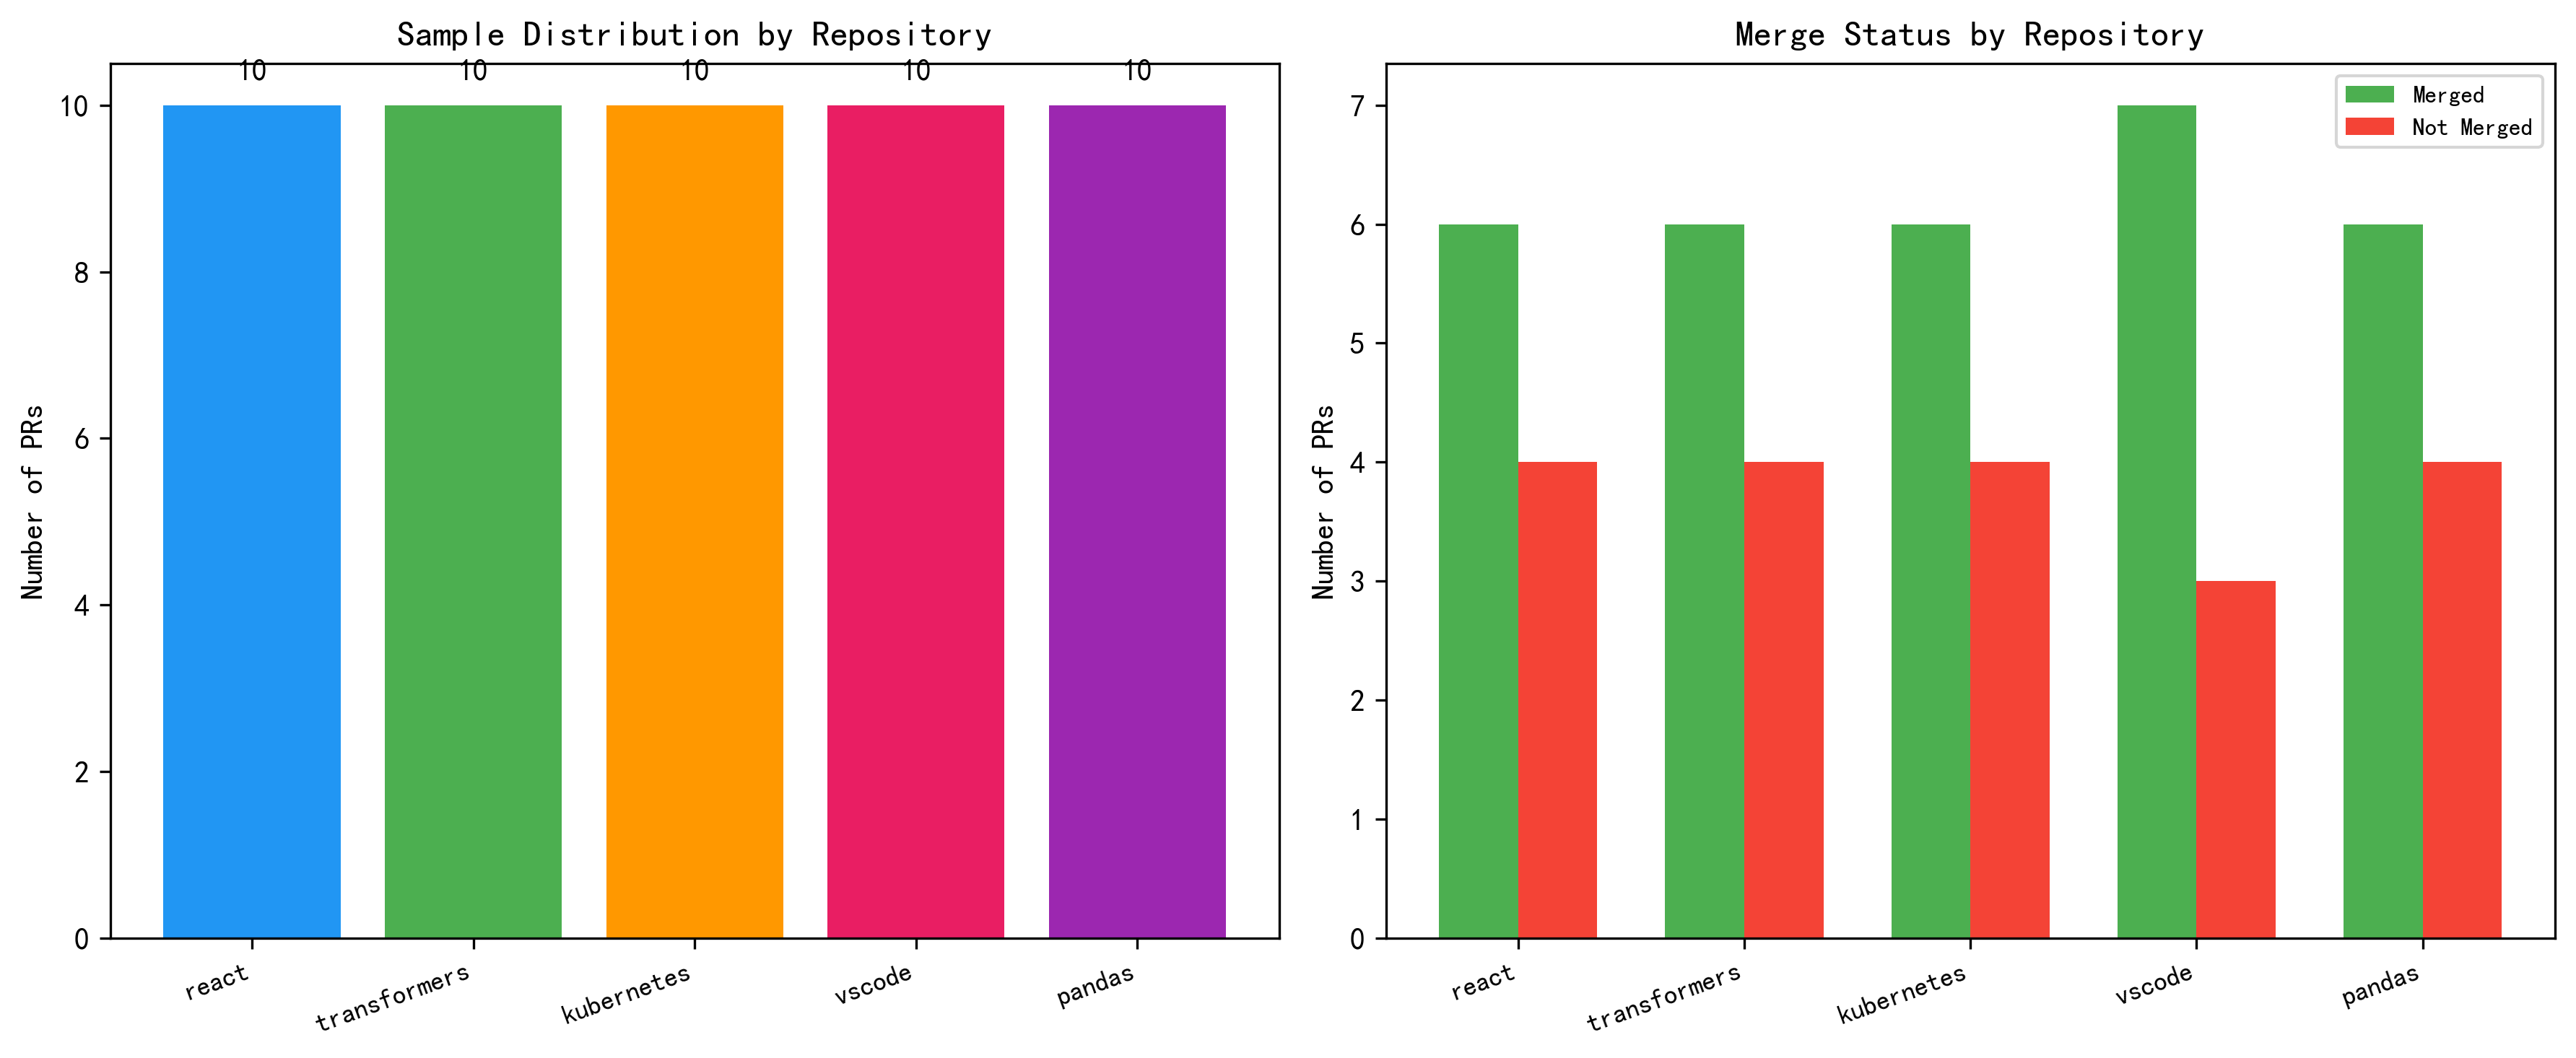
\includegraphics[width=\textwidth]{../figures/01_sample_distribution.png}
\captionof{figure}{50 条抽样 PR 的仓库分布（左）与合并状态分布（右）}
\end{center}

抽样覆盖 5 个仓库各 10 条，合并率 62.0\% 与测试集整体（64.3\%）基本一致。

\subsection*{3.2 上下文长度分析}

\begin{center}
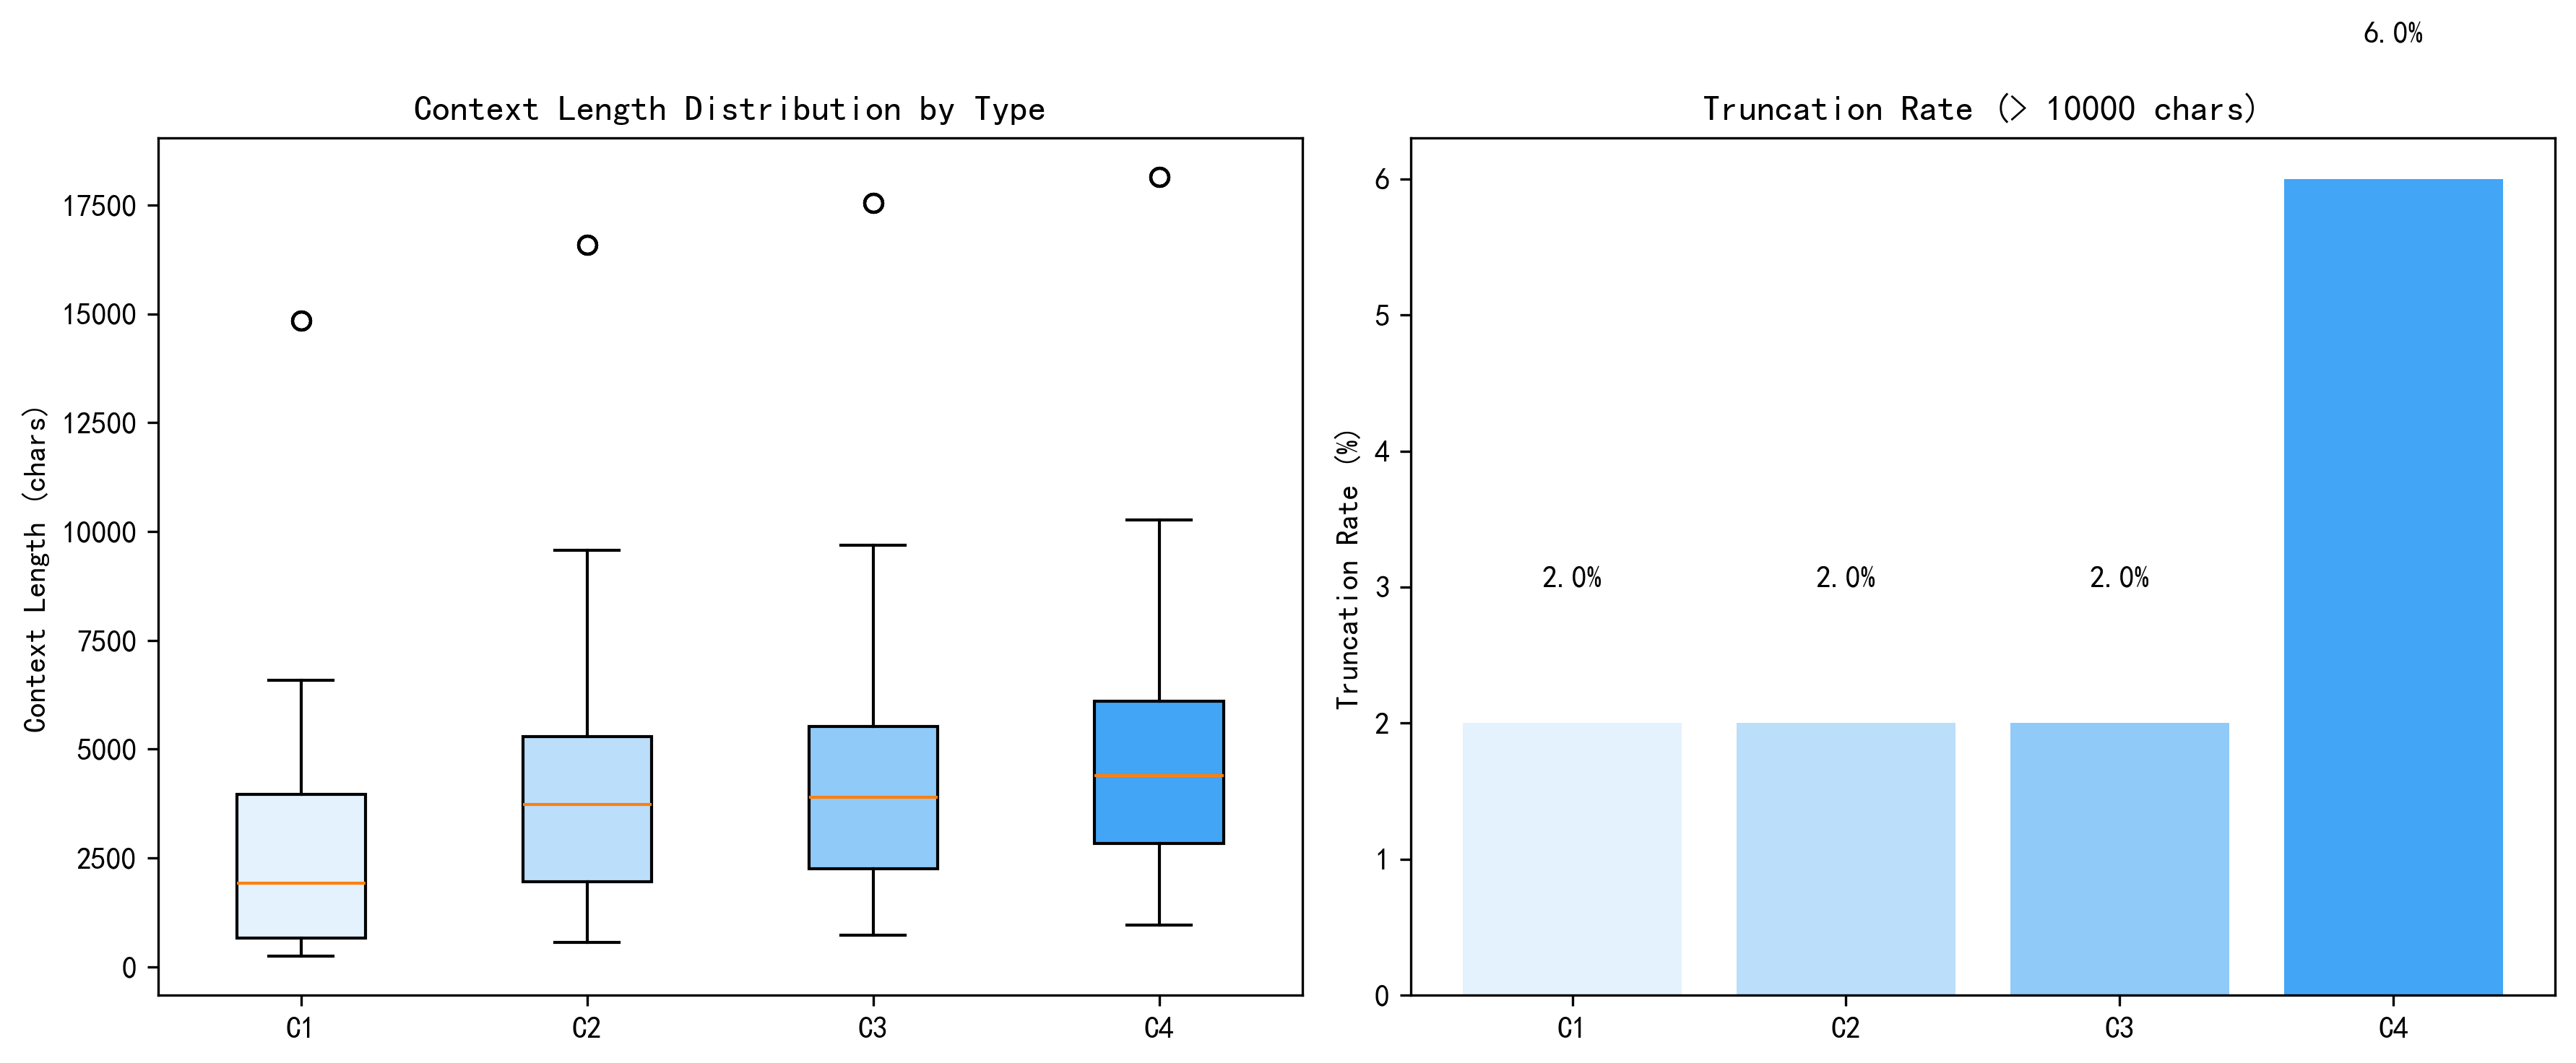
\includegraphics[width=\textwidth]{../figures/02_context_lengths.png}
\captionof{figure}{四种上下文的长度分布（左）与超长截断率（右）}
\end{center}

随着信息量从 C1 到 C4 递增，上下文长度从平均 2750 chars 增长至 4846 chars。超过 10000 chars 的比例极低（C4 仅 3/50 = 6\%），说明上下文长度整体在模型处理能力范围内，无需大规模截断。

\subsection*{3.3 Merge Prediction 结果}

\subsubsection*{3.3.1 总体指标}

16 个 Prompt $\times$ Context 组合在 50 条测试 PR 上的 Merge Prediction 指标如下：

\begin{center}
\captionof{table}{Prompt $\times$ Context 组合的 Merge Prediction 指标}
\scriptsize
\begin{tabular}{|l|l|c|c|c|c|c|c|}
\hline
\textbf{Prompt} & \textbf{Context} & \textbf{Acc} & \textbf{Prec} & \textbf{Recall} & \textbf{F1} & \textbf{AUC} & \textbf{耗时(ms)} \\
\hline
P1 Zero-shot & C1 Diff Only & 0.653 & 0.652 & 0.968 & 0.779 & 0.493 & 8664 \\
P1 Zero-shot & C2 +PR Desc  & 0.653 & 0.638 & 1.000 & 0.779 & 0.575 & 9523 \\
P1 Zero-shot & C3 +Commit   & 0.660 & 0.646 & 1.000 & 0.785 & 0.545 & 9860 \\
P1 Zero-shot & C4 Full       & 0.638 & 0.622 & 1.000 & 0.767 & 0.516 & 8985 \\
\hline
P2 Few-shot  & C1 Diff Only & 0.620 & 0.636 & 0.903 & 0.747 & 0.559 & 9483 \\
P2 Few-shot  & C2 +PR Desc  & 0.694 & 0.667 & 1.000 & 0.800 & 0.582 & 8779 \\
\rowcolor{yellow!20}
P2 Few-shot  & C3 +Commit   & \textbf{0.700} & 0.674 & 1.000 & \textbf{0.805} & 0.542 & 9577 \\
P2 Few-shot  & C4 Full       & 0.673 & 0.667 & 0.968 & 0.789 & \textbf{0.643} & 9404 \\
\hline
P3 Role      & C1 Diff Only & 0.600 & 0.649 & 0.774 & 0.706 & 0.520 & 9496 \\
P3 Role      & C2 +PR Desc  & 0.620 & 0.636 & 0.903 & 0.747 & 0.581 & 9915 \\
P3 Role      & C3 +Commit   & 0.592 & 0.614 & 0.900 & 0.730 & 0.508 & 8601 \\
P3 Role      & C4 Full       & 0.612 & 0.636 & 0.903 & 0.747 & 0.562 & 8606 \\
\hline
P4 CoT       & C1 Diff Only & 0.660 & 0.646 & 1.000 & 0.785 & 0.544 & 9130 \\
P4 CoT       & C2 +PR Desc  & 0.646 & 0.644 & 0.967 & 0.773 & 0.551 & 9466 \\
P4 CoT       & C3 +Commit   & 0.660 & 0.646 & 1.000 & 0.785 & 0.531 & 10025 \\
P4 CoT       & C4 Full       & 0.673 & 0.660 & 1.000 & 0.795 & 0.474 & 9182 \\
\hline
\end{tabular}
\end{center}

\subsubsection*{3.3.2 热力图分析}

\begin{center}
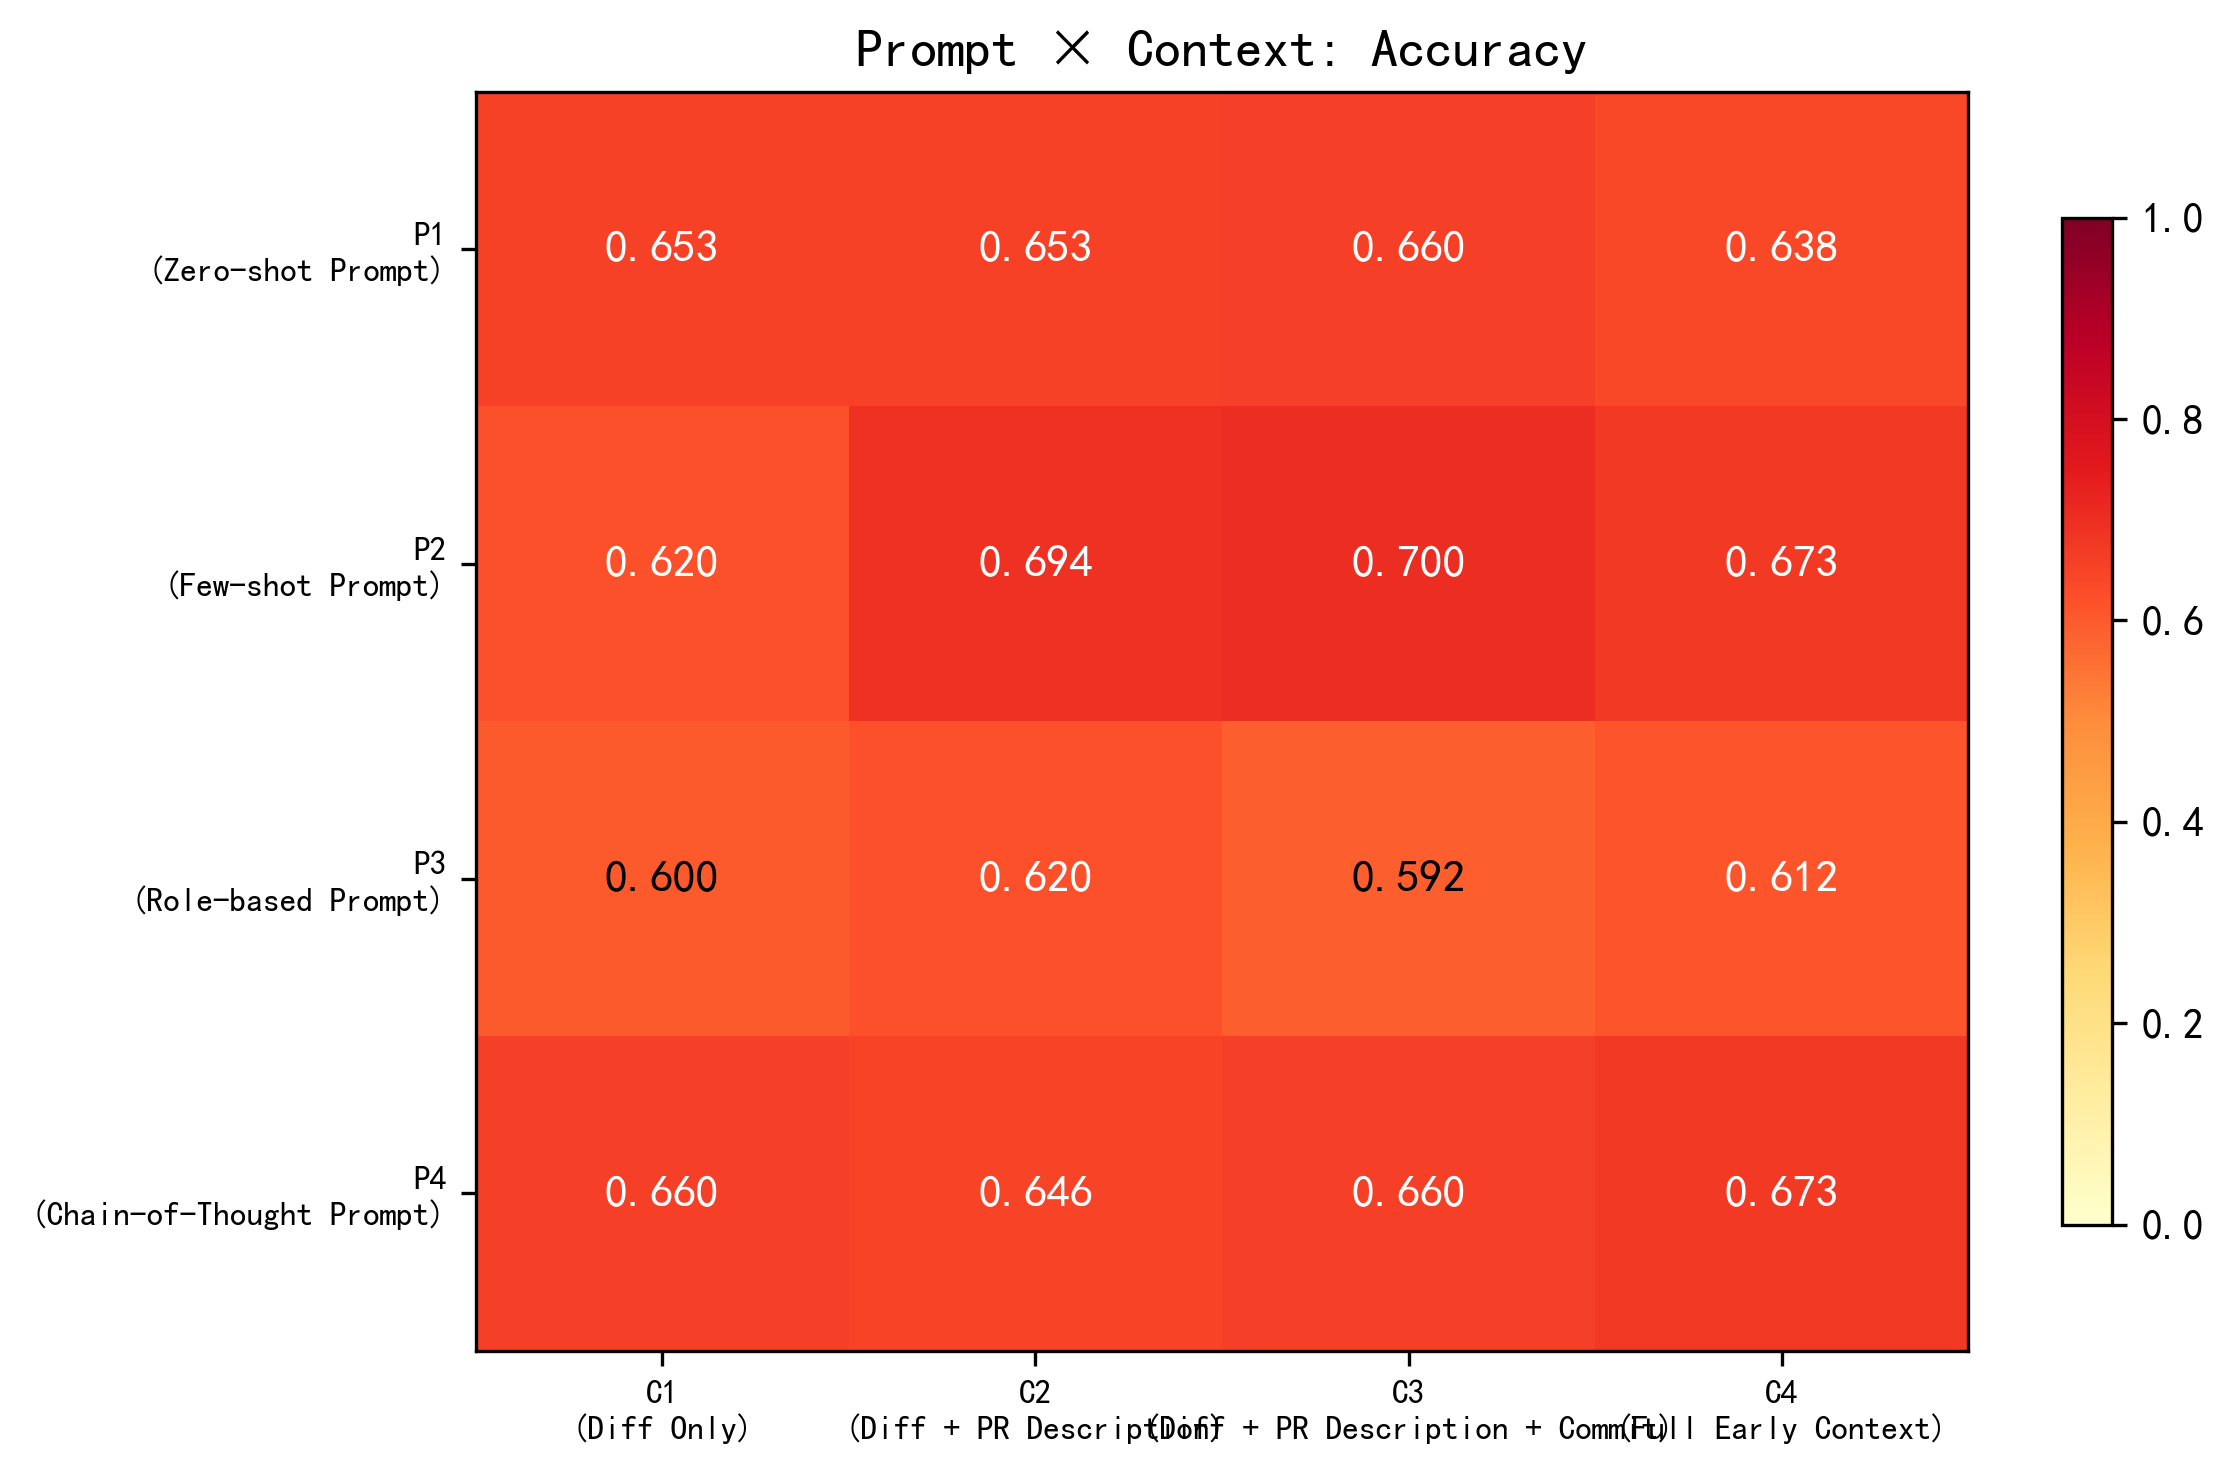
\includegraphics[width=0.48\textwidth]{../figures/03_accuracy_heatmap.png}
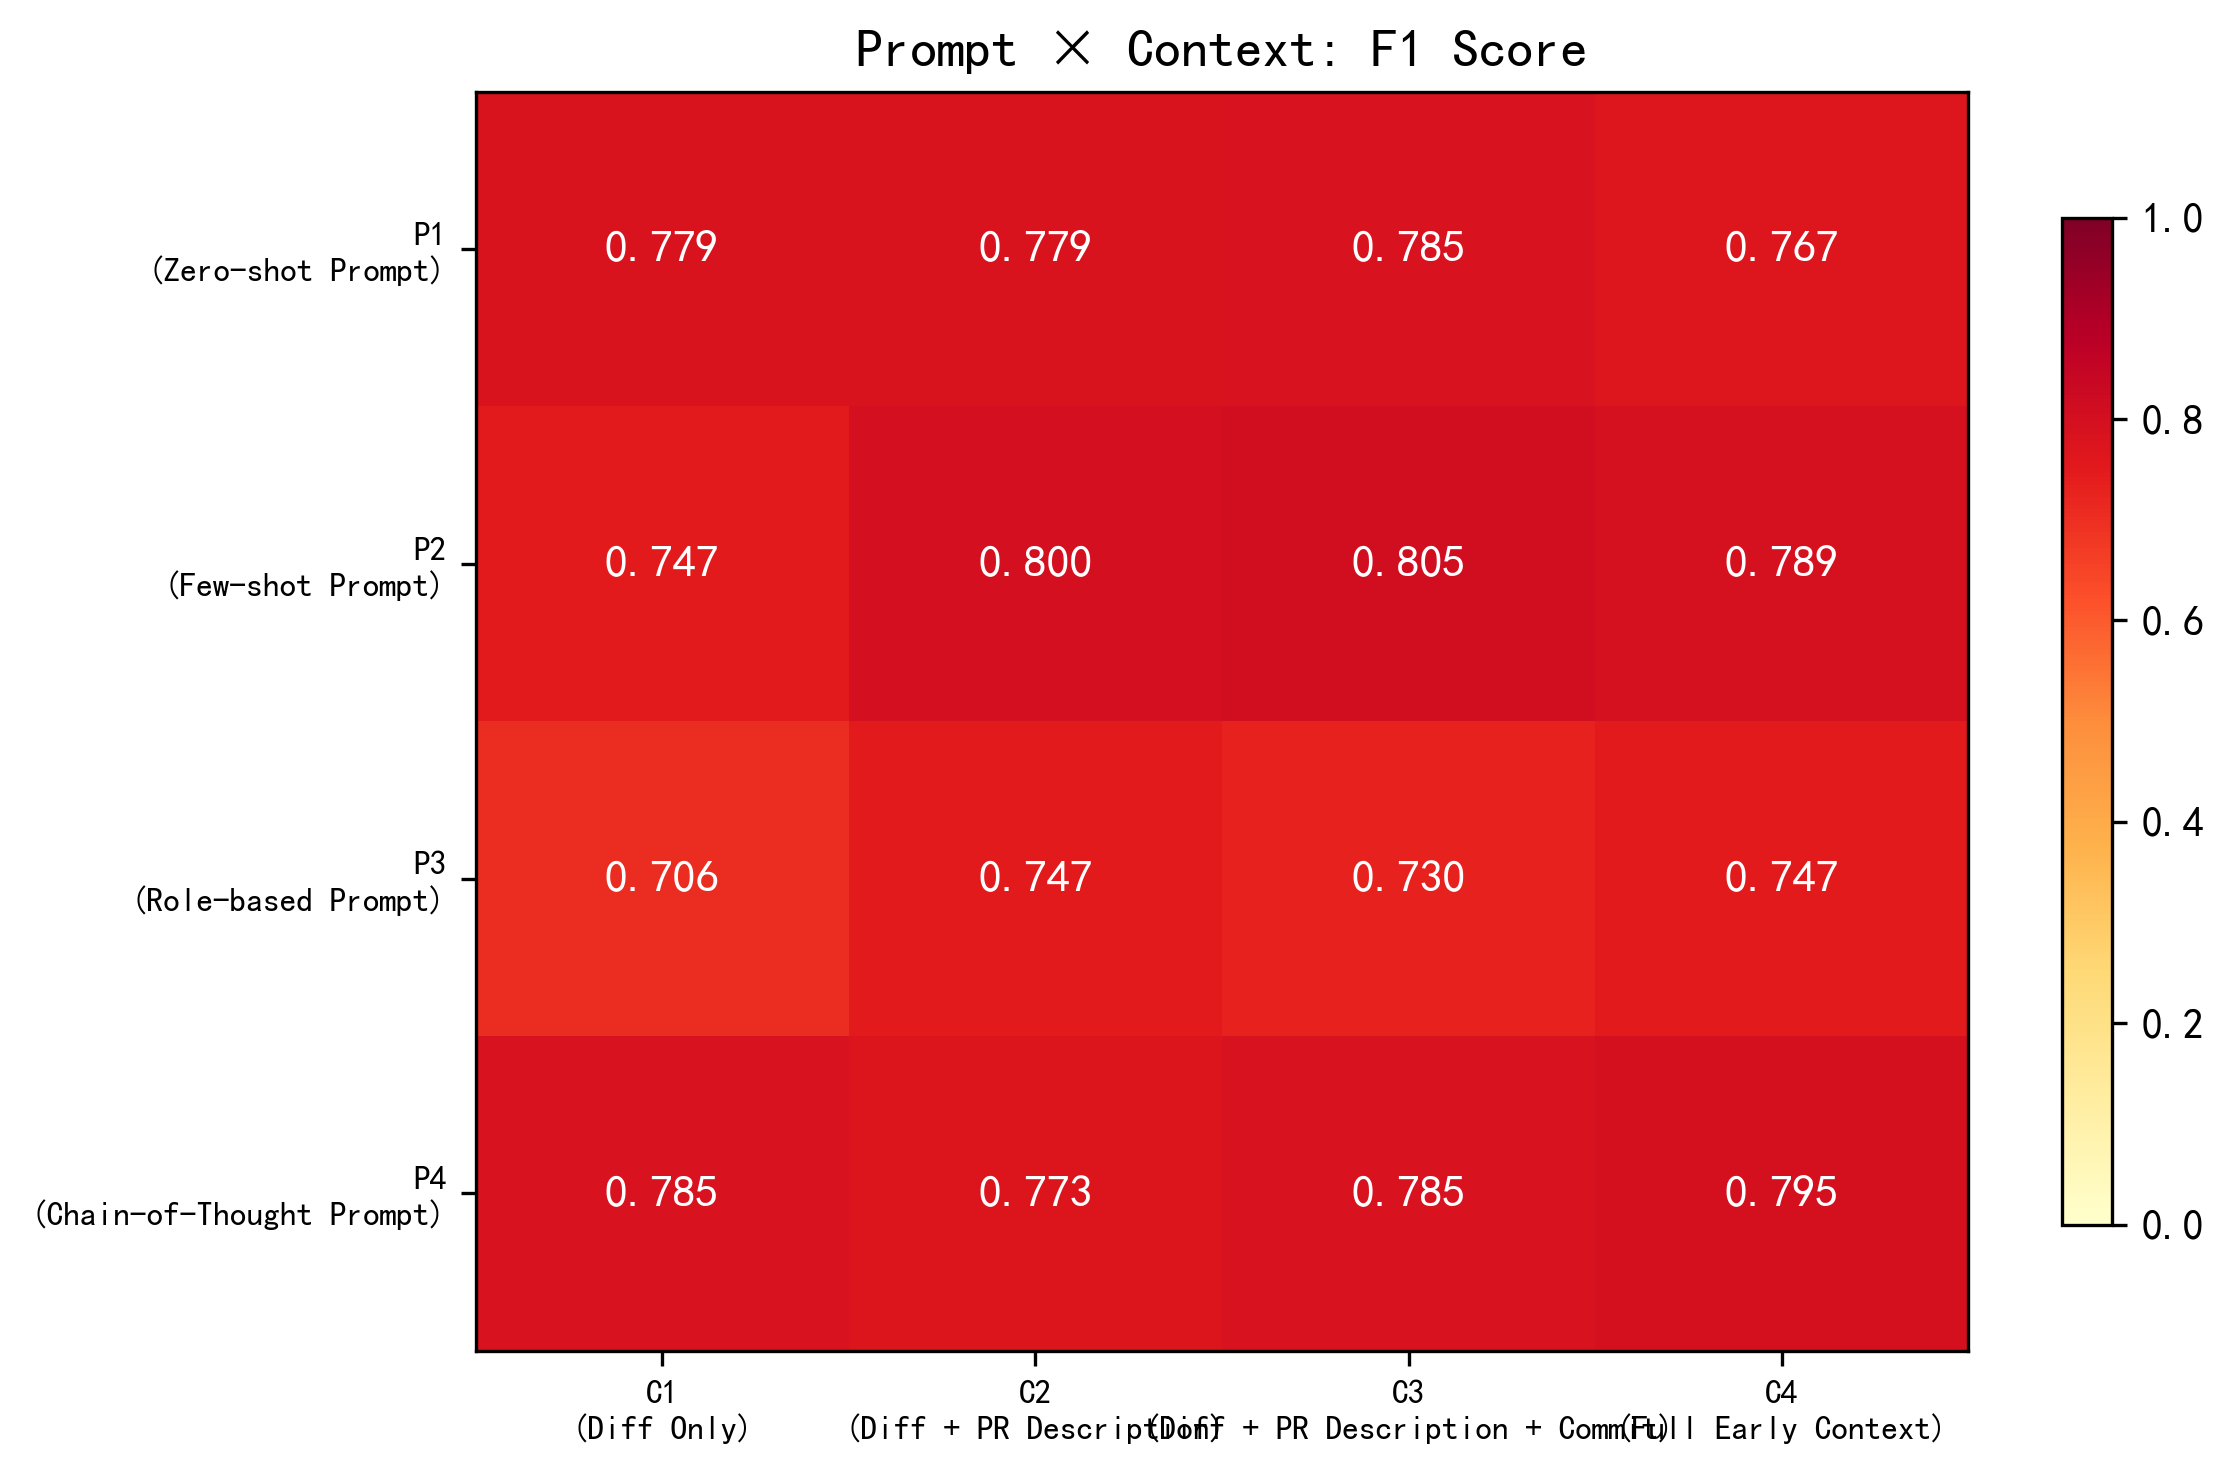
\includegraphics[width=0.48\textwidth]{../figures/04_f1_heatmap.png}
\captionof{figure}{Accuracy（左）与 F1-score（右）热力图}
\end{center}

\begin{center}
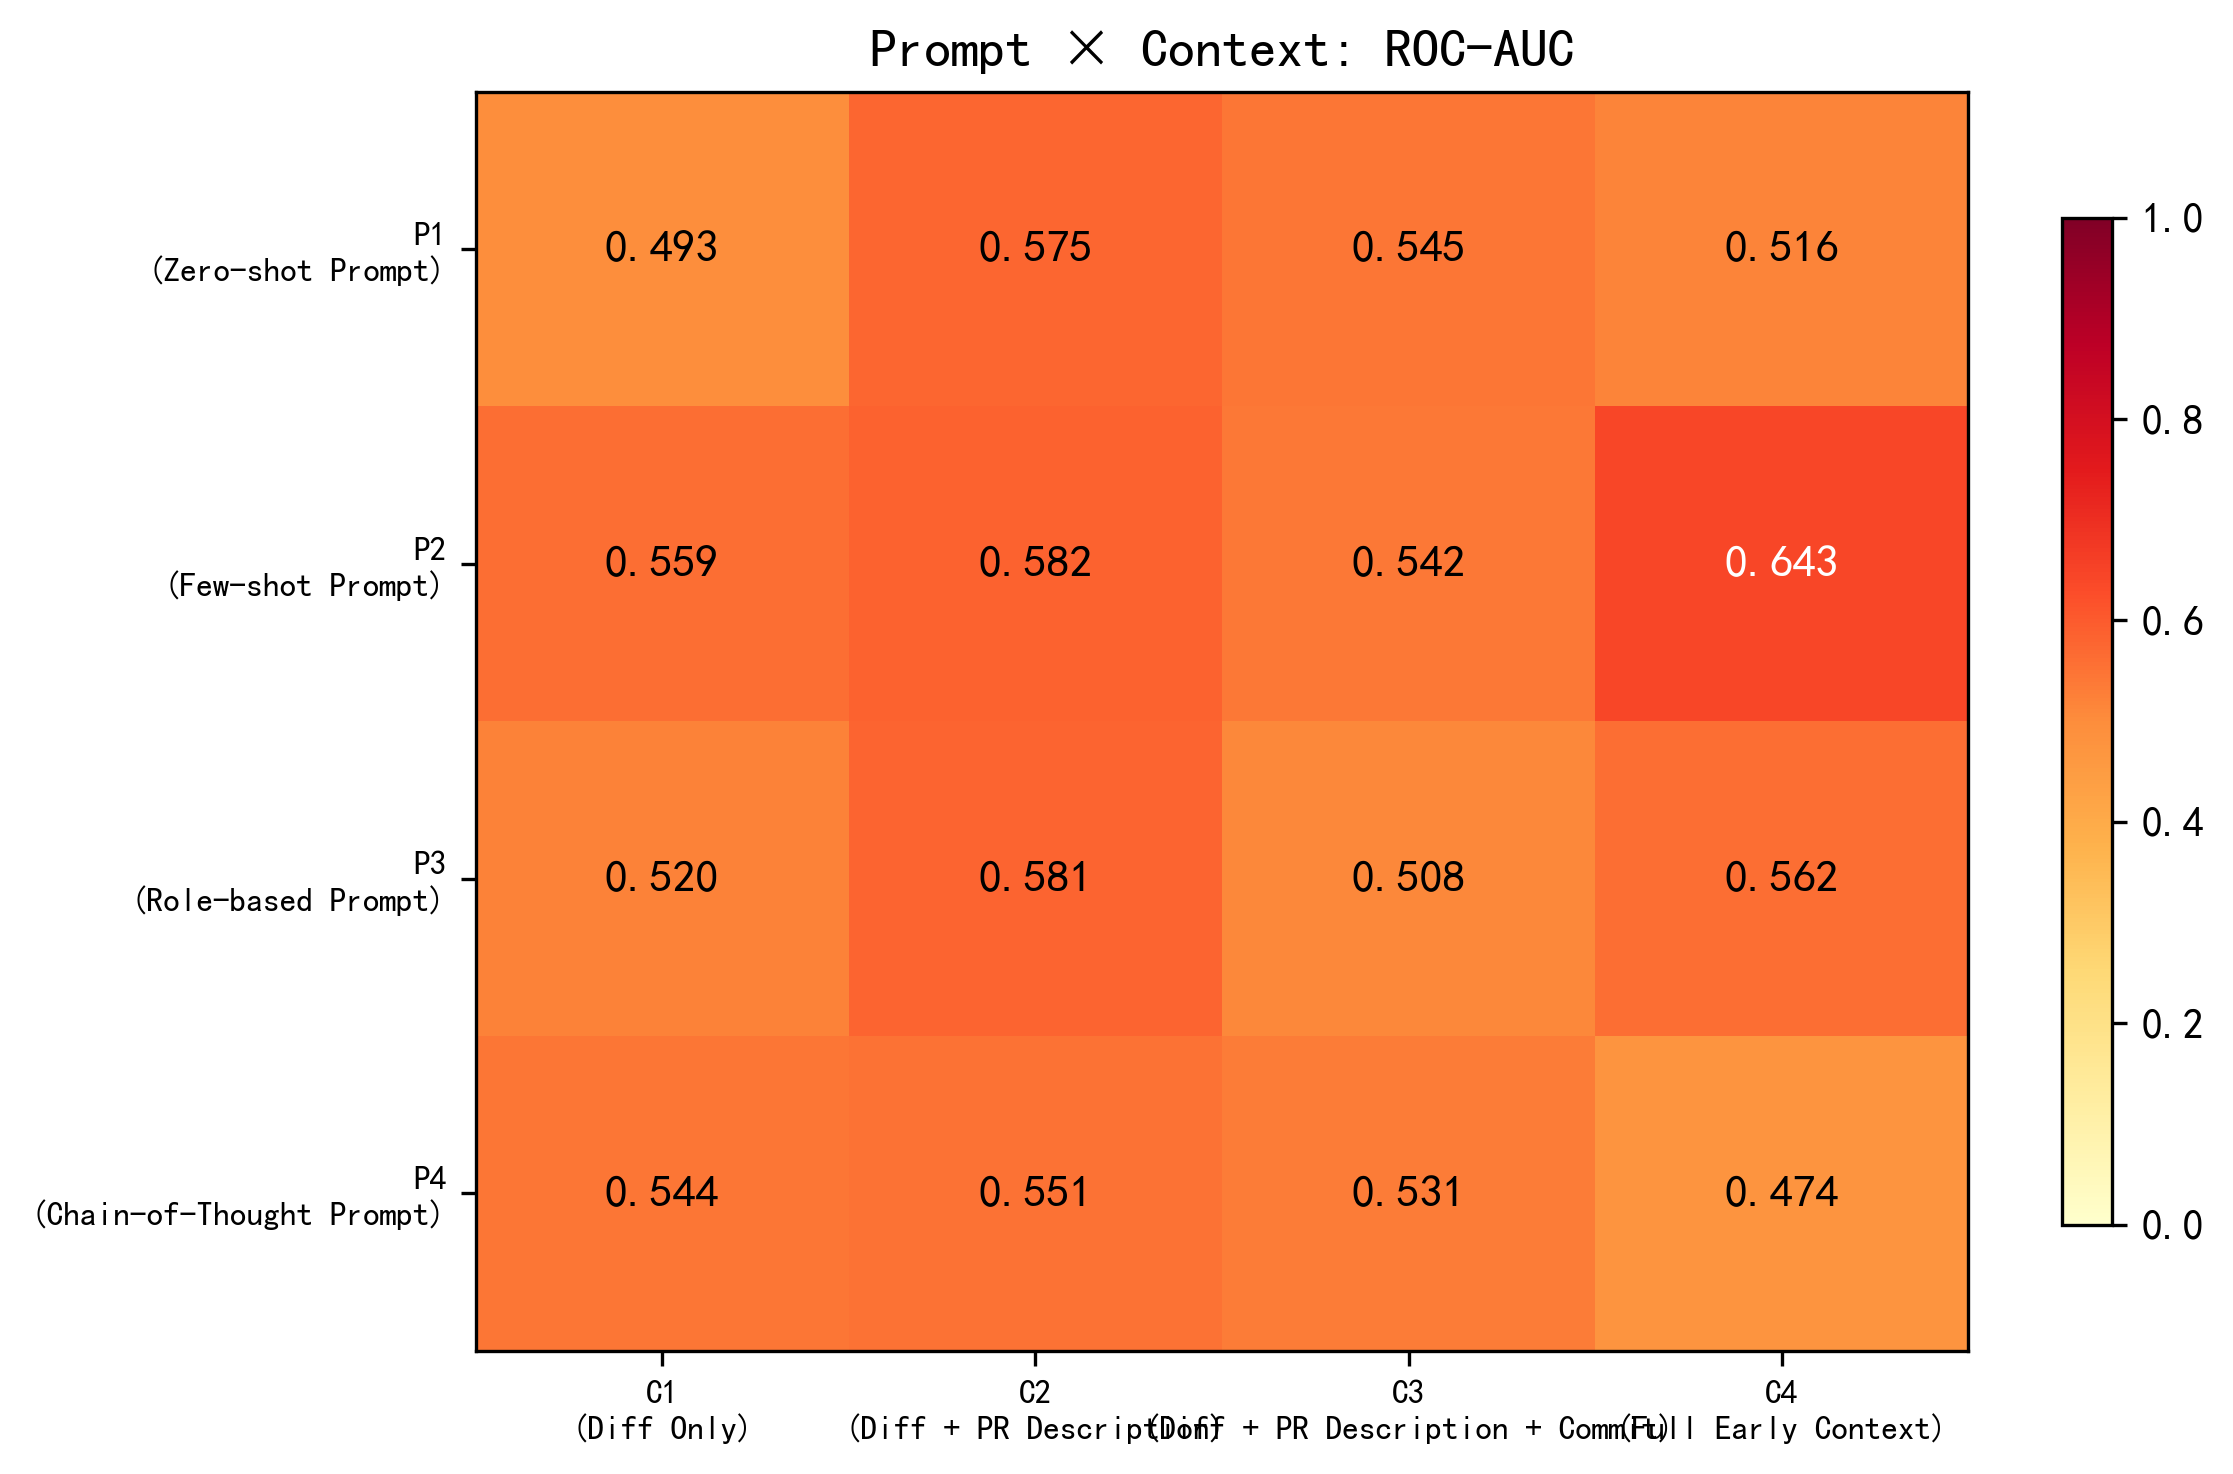
\includegraphics[width=0.48\textwidth]{../figures/05_roc_auc_heatmap.png}
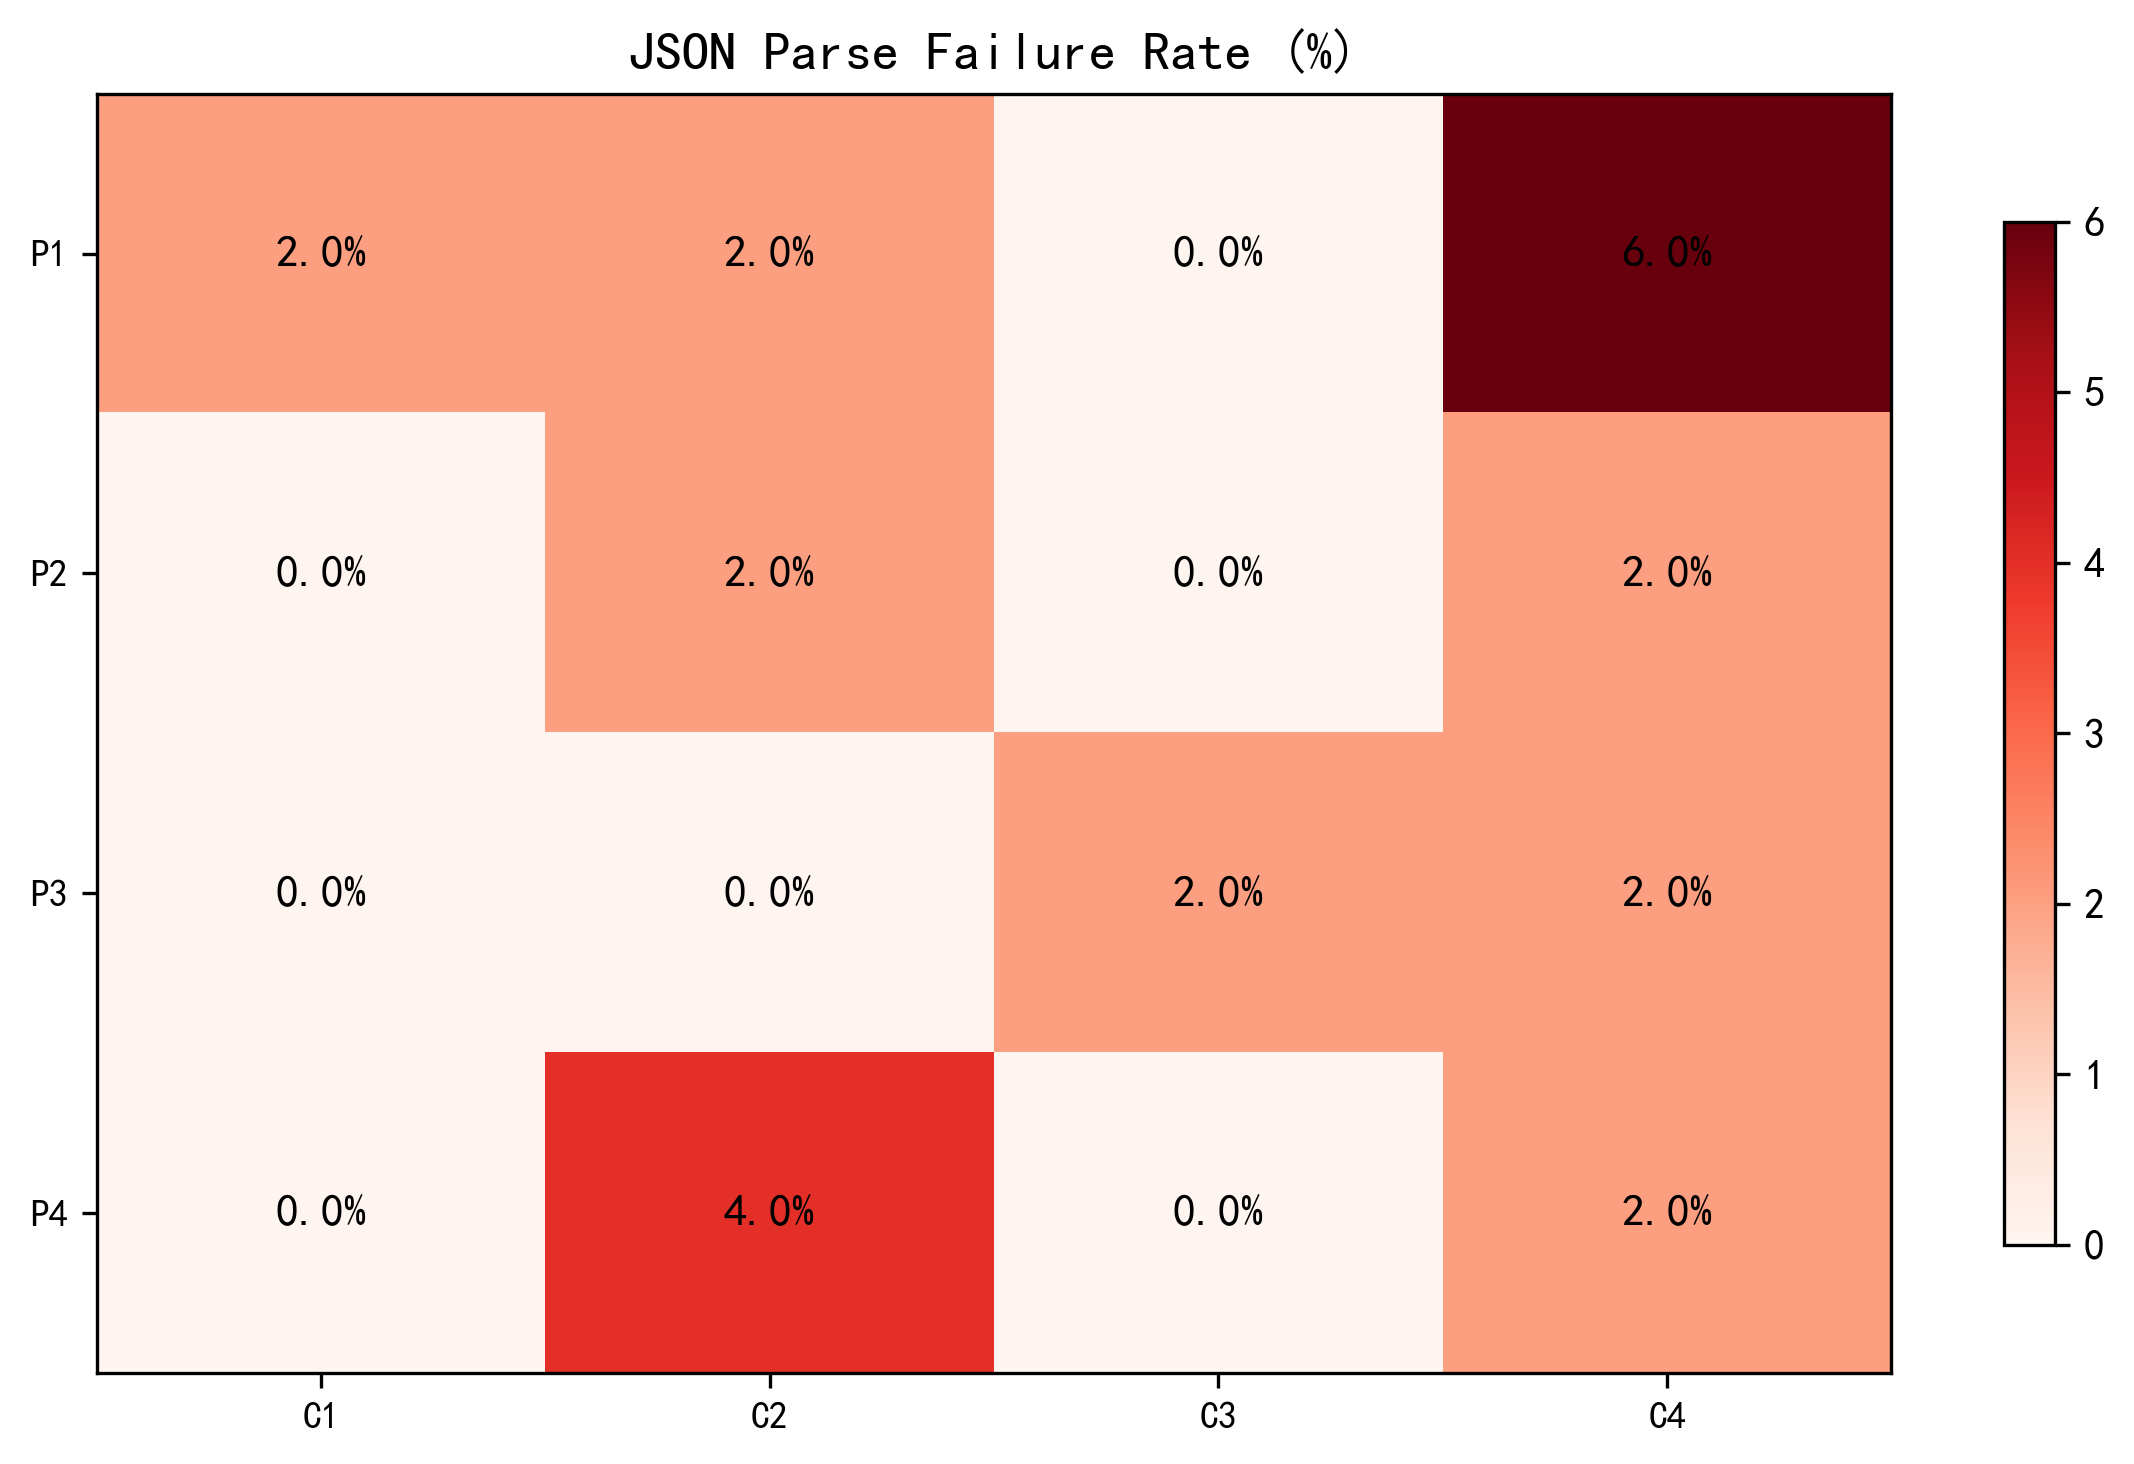
\includegraphics[width=0.48\textwidth]{../figures/09_parse_fail_rate.png}
\captionof{figure}{ROC-AUC（左）与 JSON 解析失败率（右）热力图}
\end{center}

\subsubsection*{3.3.3 关键发现}

\textbf{（1）最佳组合：P2/C3（Few-shot + Diff+PR+Commit）}取得最高 F1（0.8052）和 Accuracy（0.7000），验证了 Few-shot 示例对任务理解有帮助，且 C3 级别的上下文信息量（包含 diff、PR 描述和 commit messages）达到了性能与成本的较好平衡。

\textbf{（2）P2（Few-shot）整体表现最优}，F1 均值为 0.785，高于 P1（0.778）、P4（0.785，持平）和 P3（0.732）。P3（Role-based）在所有上下文中均表现最差，可能是因为角色设定使模型过于保守，产生了更多 False Positive。

\textbf{（3）上下文信息量的边际收益有限。}从 C1 到 C3，F1 从 0.754 增至 0.776（+2.2pp），但 C3 到 C4 几乎无增量。AST/CFG 摘要对 LLM 的贡献有限——LLM 已经在代码理解方面足够强大，结构化摘要提供的新信息不多。

\textbf{（4）Recall 非常高（多数组合 0.90--1.00），但 Precision 偏低（0.61--0.67）。}模型倾向于预测"合并"，导致 FP 较高（平均 16 个）、TN 很低（平均 2-4 个）。这一偏斜倾向可能源于模型在训练数据中看到了更高的合并率。

\textbf{（5）ROC-AUC 偏低（0.47--0.64），}主要原因是模型输出的 merge\_probability 区分度不足——大多数预测概率集中在 0.80--0.95 之间，即使对实际未合并的 PR 也给出了高概率。

\subsection*{3.4 Review Comment Generation 结果}

\begin{center}
\captionof{table}{Review Comment Generation 指标（45 条有真实评论的 PR）}
\scriptsize
\begin{tabular}{|l|l|c|c|c|c|c|}
\hline
\textbf{Prompt} & \textbf{Context} & \textbf{BLEU} & \textbf{ROUGE-1} & \textbf{ROUGE-2} & \textbf{ROUGE-L} & \textbf{均评论数} \\
\hline
P1 & C1 & 0.0000 & 0.1163 & 0.0081 & 0.0744 & 2.61 \\
P1 & C2 & 0.0000 & 0.1127 & 0.0094 & 0.0736 & 2.93 \\
P1 & C3 & 0.0000 & 0.1212 & 0.0112 & \textbf{0.0760} & 2.82 \\
P1 & C4 & 0.0000 & 0.1172 & 0.0100 & 0.0712 & 2.74 \\
\hline
P2 & C1 & 0.0000 & 0.1057 & 0.0070 & 0.0674 & 2.20 \\
P2 & C2 & 0.0006 & 0.1086 & 0.0104 & 0.0703 & 2.27 \\
P2 & C3 & \textbf{0.0006} & 0.1133 & 0.0093 & 0.0725 & 2.62 \\
P2 & C4 & 0.0000 & 0.1056 & 0.0110 & 0.0707 & 2.41 \\
\hline
P3 & C1 & 0.0000 & 0.0897 & 0.0064 & 0.0552 & 1.64 \\
P3 & C2 & 0.0000 & 0.1070 & 0.0091 & 0.0653 & 1.67 \\
P3 & C3 & 0.0006 & 0.1137 & 0.0096 & 0.0720 & 1.73 \\
P3 & C4 & 0.0000 & 0.1168 & 0.0109 & 0.0694 & 1.45 \\
\hline
P4 & C1 & 0.0000 & 0.0960 & 0.0047 & 0.0595 & 2.02 \\
P4 & C2 & 0.0000 & 0.0927 & 0.0054 & 0.0588 & 1.77 \\
P4 & C3 & 0.0000 & 0.1093 & 0.0085 & 0.0695 & 1.87 \\
P4 & C4 & 0.0000 & 0.1061 & 0.0082 & 0.0702 & 1.93 \\
\hline
\end{tabular}
\end{center}

\begin{center}
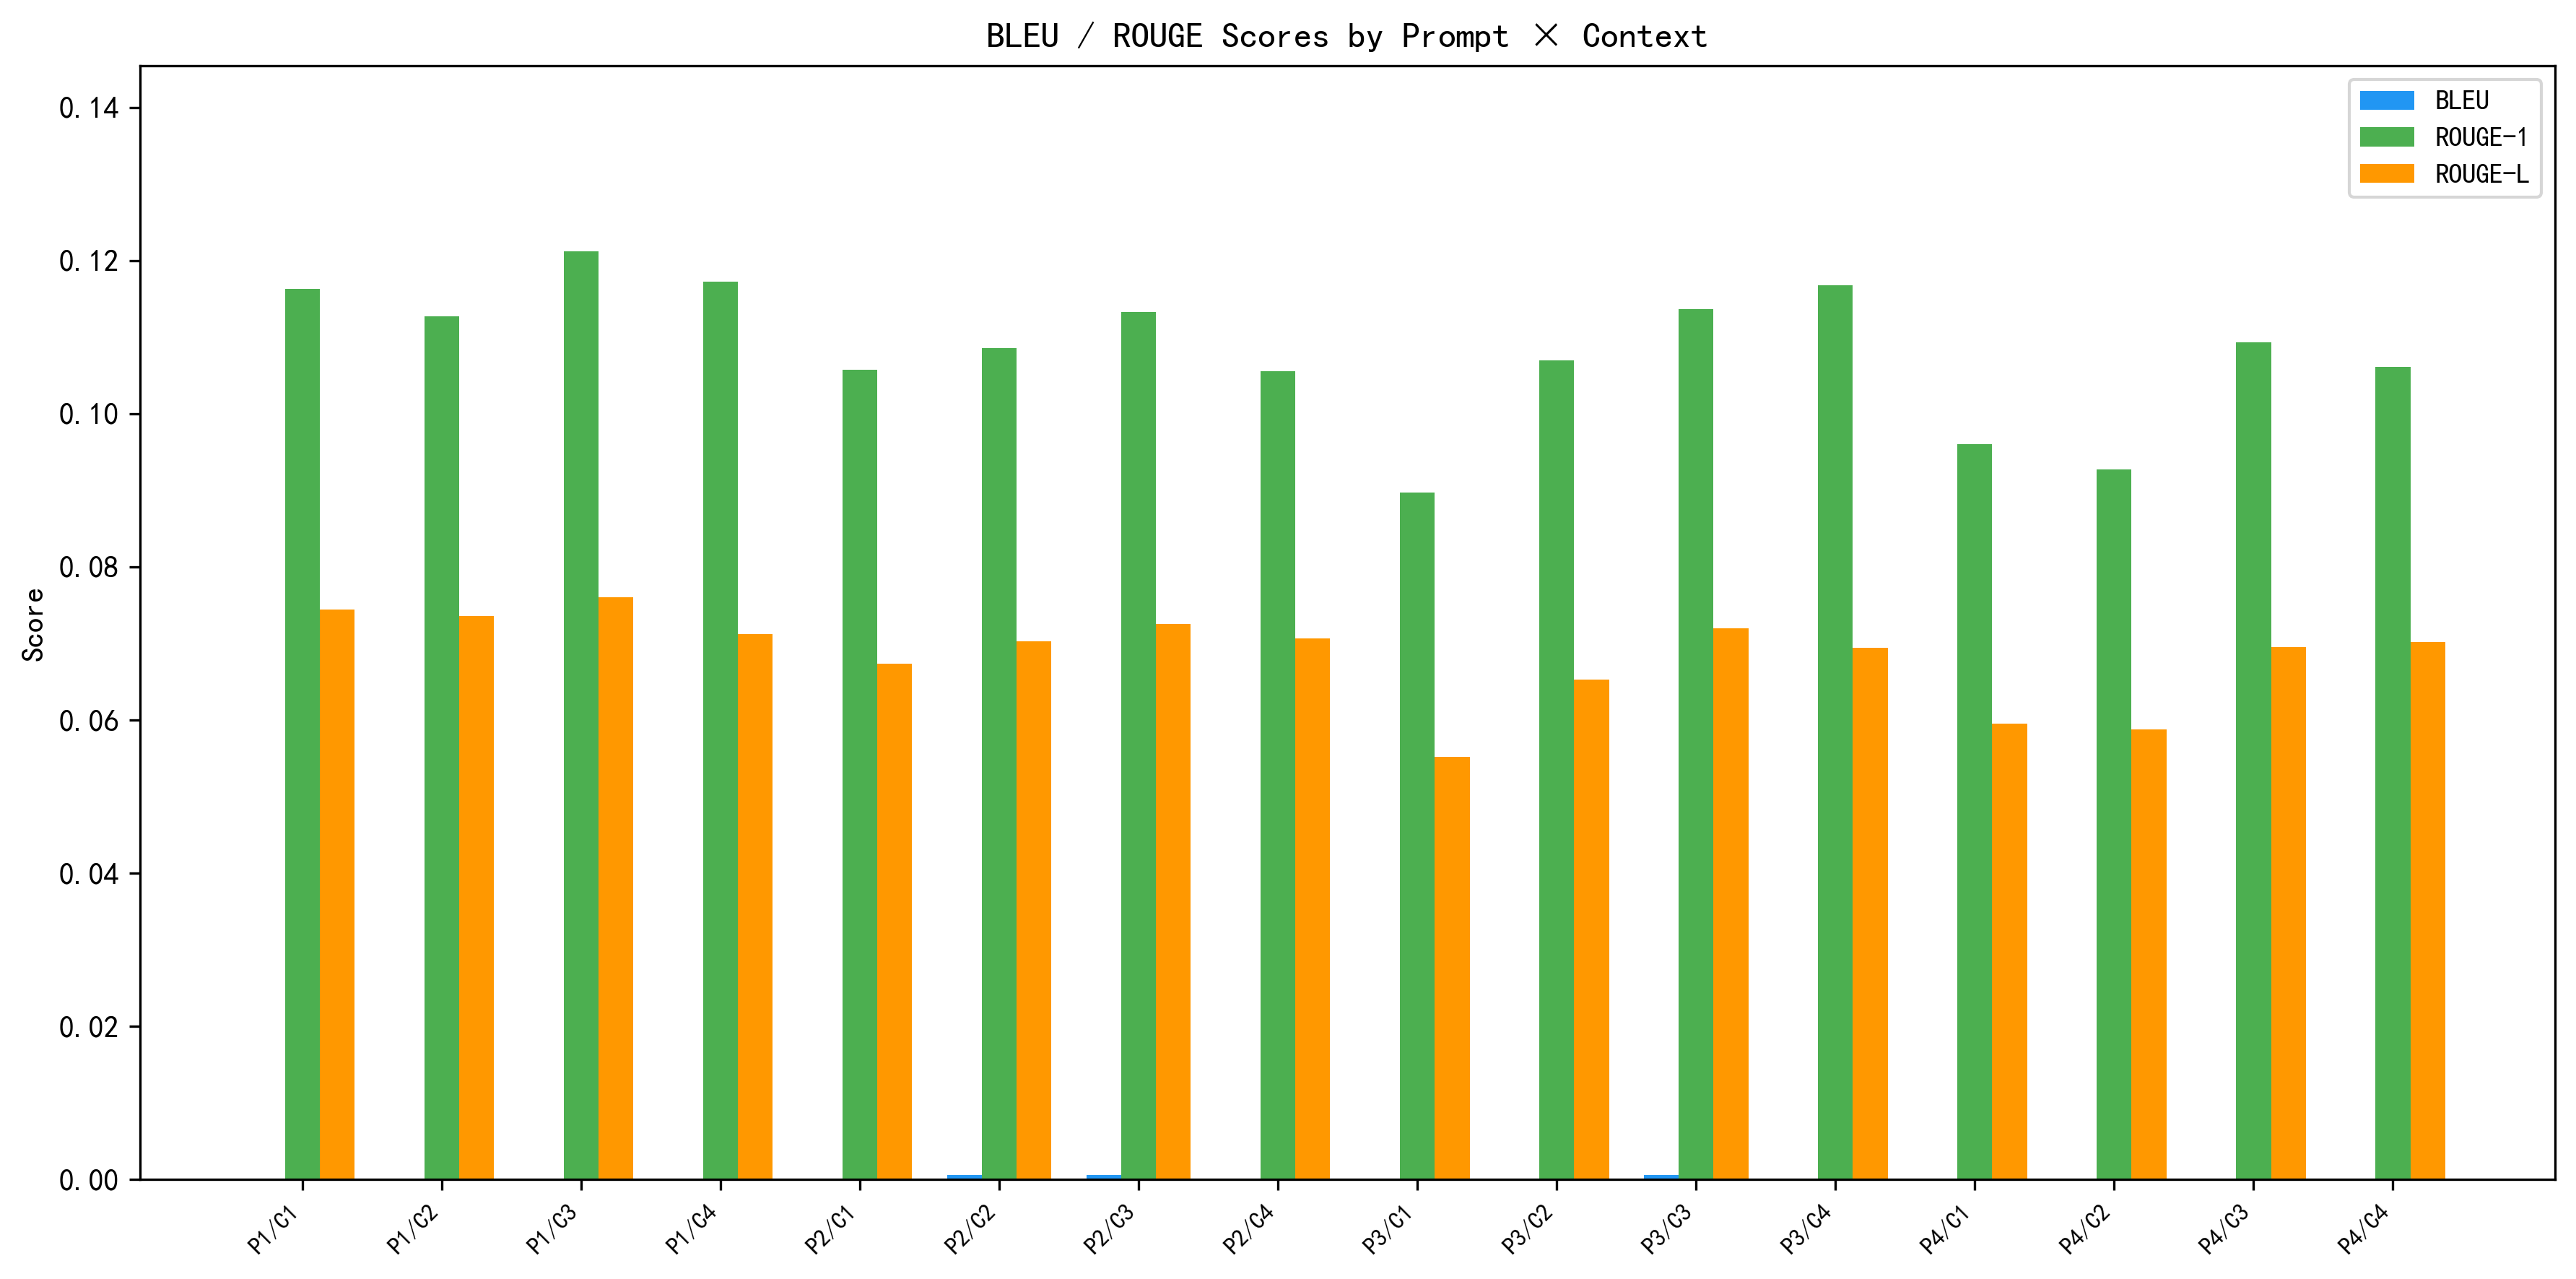
\includegraphics[width=\textwidth]{../figures/06_bleu_rouge_comparison.png}
\captionof{figure}{BLEU / ROUGE 分数对比}
\end{center}

\textbf{关键发现：}

\textbf{（1）BLEU 接近 0，ROUGE-L 在 0.055--0.076 之间。}这是预期之内的结果——BLEU 衡量 n-gram 精确匹配，LLM 生成的评论用词、句式和关注点与人类 Reviewer 几乎不可能逐词一致。ROUGE-L 基于最长公共子序列，约为 0.07，表明生成评论与真实评论在词序列层面有微弱但非零的关联。

\textbf{（2）P1 生成评论最多（平均 2.61--2.93 条），P3 最少（1.45--1.73 条）。}P1 更"自由"，P3 的 maintainer 角色设定使模型更审慎，倾向于减少评论数量。

\textbf{（3）Severity 分布：}整体 1687 条生成评论中，nit 占 46.8\%，minor 占 43.5\%，major 占 6.8\%，blocker 占 2.7\%，分布较为合理——大部分评论为建议性（nit/minor），阻断性评论（blocker）较少。

\textbf{（4）空参考样本（无真实 review text）仍生成评论：}5 条无真实评论的 PR 中，80 次调用中有 68 次仍生成了 review comments，说明 LLM 在无参照时仍倾向于给出反馈。

\subsection*{3.5 推理时间分析}

\begin{center}
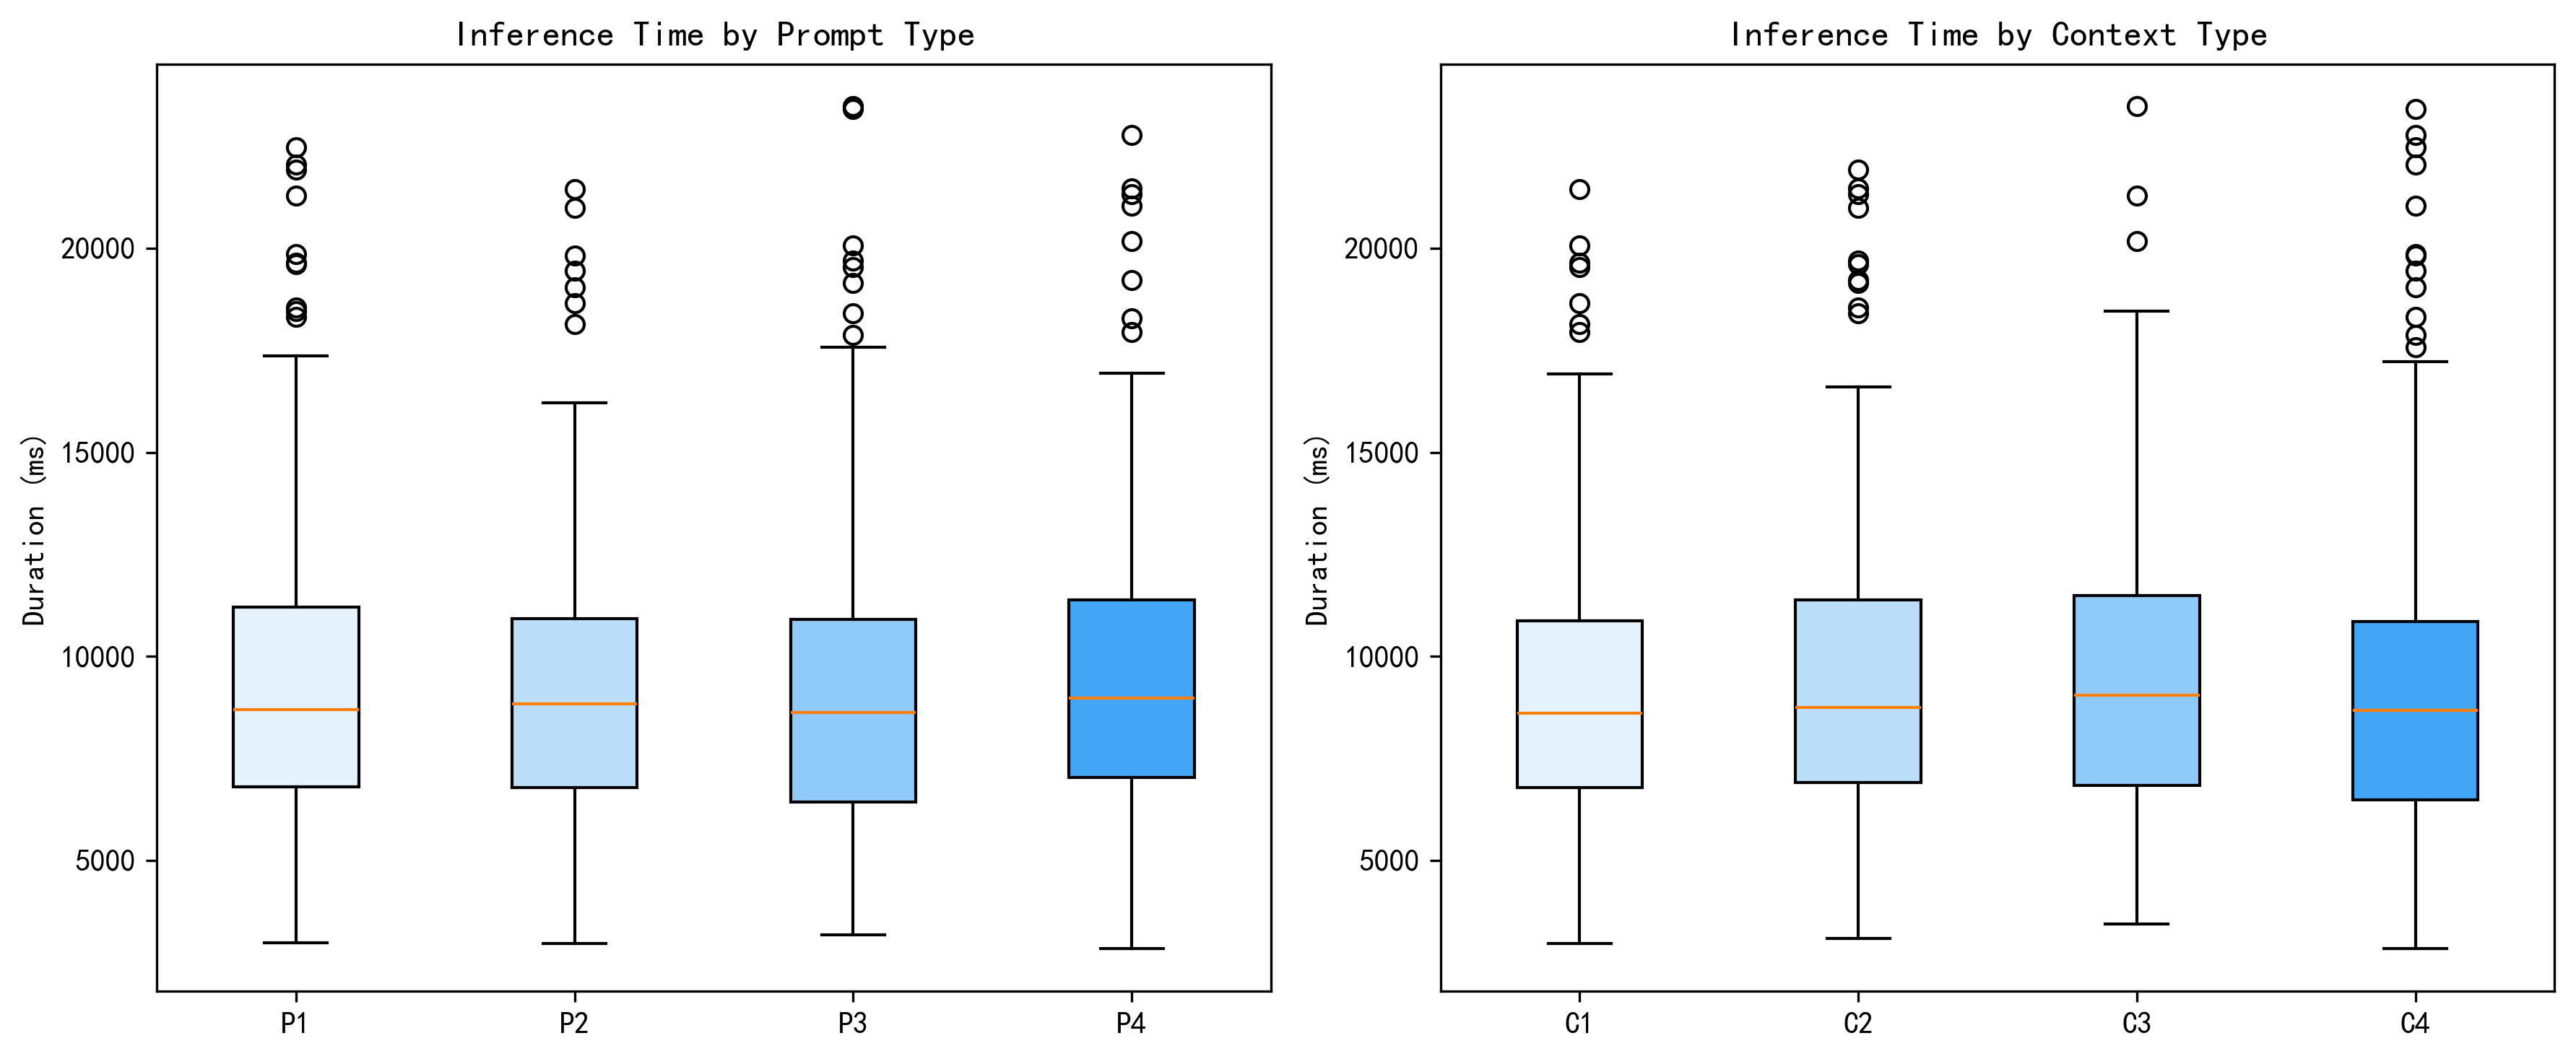
\includegraphics[width=\textwidth]{../figures/07_inference_time.png}
\captionof{figure}{推理时间按 Prompt 类型（左）和 Context 类型（右）对比}
\end{center}

平均推理时间约 9.5 秒/条，各 Prompt 和 Context 类型之间差异不大（范围 8600--10000 ms）。采用 8 并发后，800 次调用总耗时约 15 分钟，平均有效吞吐量约 0.85 条/秒。

\subsection*{3.6 与实验二传统机器学习对比}

\begin{center}
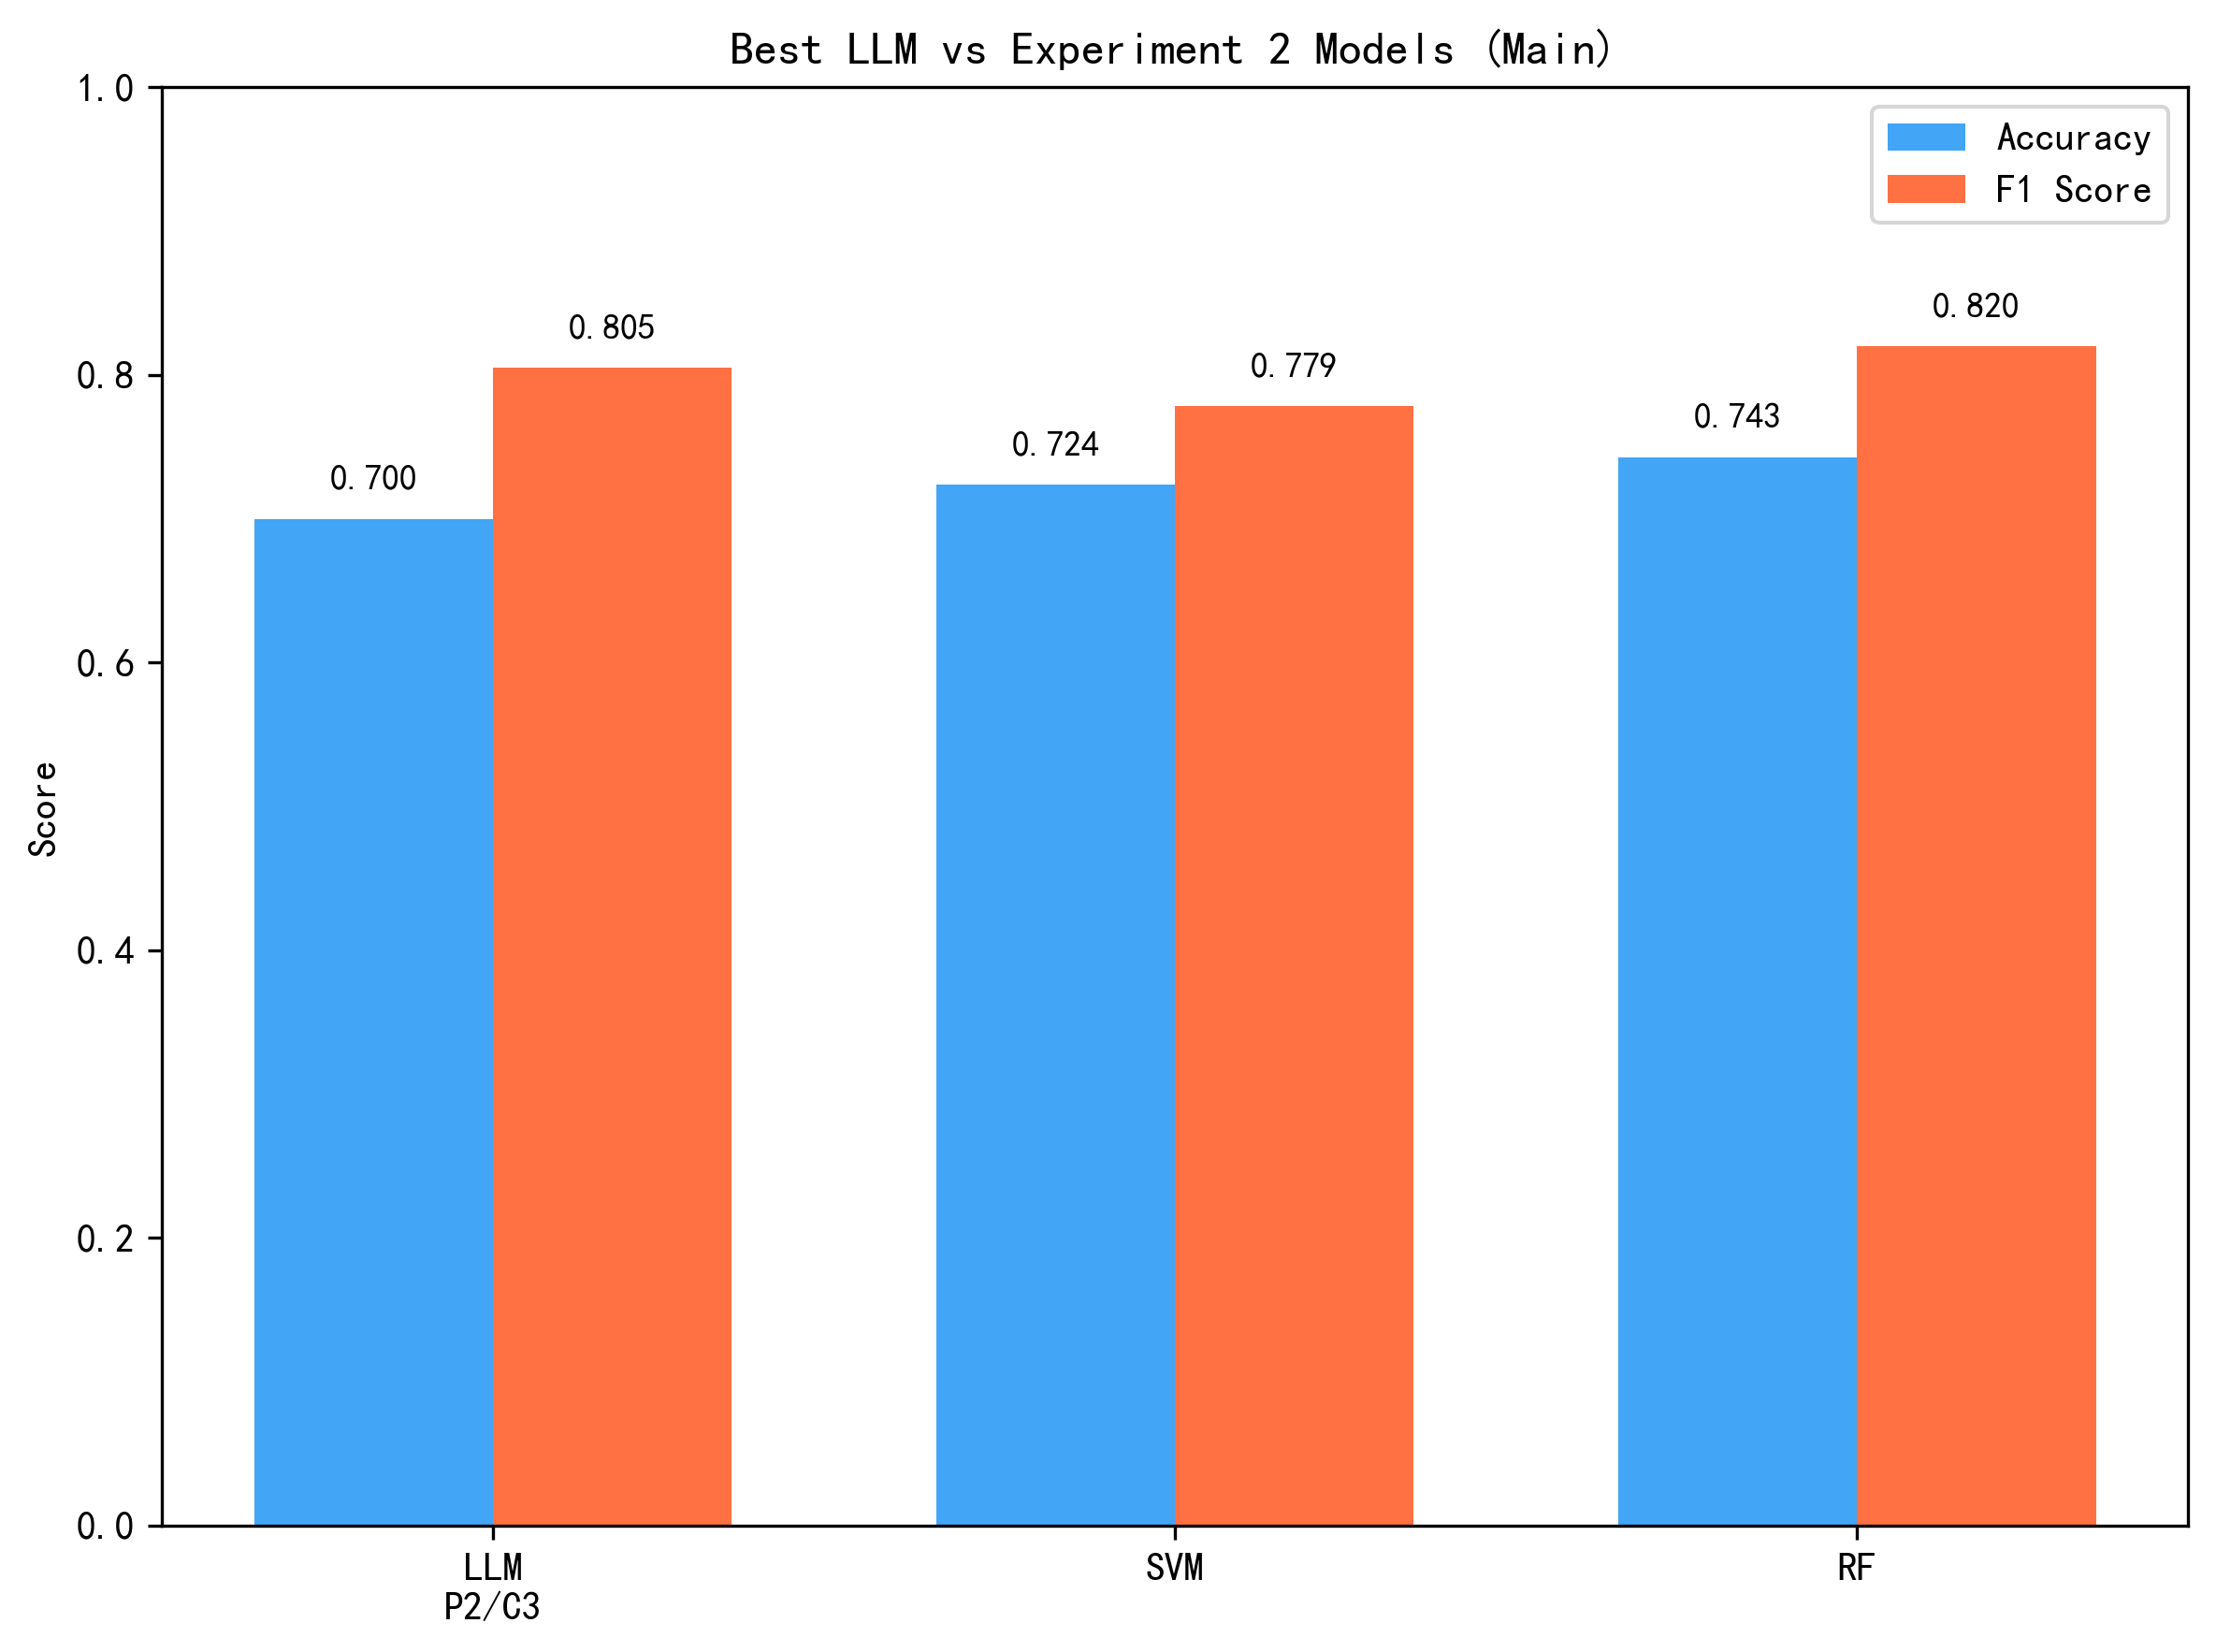
\includegraphics[width=0.65\textwidth]{../figures/08_model_comparison.png}
\captionof{figure}{最佳 LLM 组合（P2/C3）与实验二传统模型对比}
\end{center}

\begin{center}
\captionof{table}{LLM vs 传统机器学习对比}
\begin{tabular}{|l|c|c|c|c|c|}
\hline
\textbf{方法} & \textbf{Accuracy} & \textbf{Precision} & \textbf{Recall} & \textbf{F1} & \textbf{AUC} \\
\hline
Dummy (most\_frequent) & 0.643 & -- & -- & 0.783 & 0.500 \\
SVM（实验二主实验）             & 0.724 & \textbf{0.803} & 0.756 & 0.779 & 0.779 \\
Random Forest（实验二主实验）    & \textbf{0.743} & 0.746 & \textbf{0.911} & \textbf{0.820} & \textbf{0.806} \\
\hline
LLM P2/C3（本实验）             & 0.700 & 0.674 & 1.000 & 0.805 & 0.542 \\
\hline
\end{tabular}
\end{center}

\textbf{分析：}
\begin{itemize}
    \item LLM（P2/C3）的 F1（0.805）接近 Random Forest（0.820），优于 SVM（0.779），说明 LLM 在无训练的情况下达到了与传统 ML 接近的预测能力；
    \item LLM 的 Recall（1.000）极高但 Precision（0.674）较低，说明 LLM 倾向于"宁可错杀不可放过"——将所有样本预测为 merged。这一倾向与 LLM 的训练数据分布有关；
    \item LLM 的 ROC-AUC（0.542）明显低于传统 ML（RF 0.806），核心原因是 LLM 输出的 merge\_probability 缺乏区分度。这是 zero/few-shot 设置下的固有限制——模型没有被 fine-tuned 来校准概率；
    \item \textbf{重要的是：}LLM 与实验二\textbf{主实验}（不含审查过程特征）对比是公平的。如果与实验二\textbf{上界实验}（RF AUC 0.955）对比则不公平，因为上界实验使用了审查后信息。
\end{itemize}

}

\clearpage

%========================
% 实验中遇到的问题
%========================

\experimentproblems{

\subsection*{4.1 为什么 LLM 的 Merge Prediction 需要严格限制输入信息？}

PR 刚提交时的真实场景中，系统无法获知审查结论。如果不加限制地将 \texttt{is\_merged}、\texttt{review\_decision}、\texttt{approved} 等后验信息放入 prompt，模型会学到"被 approved 的 PR 更可能合并"这种后验规律——在测试集上分数很高，但实际部署时完全不可用。实验二的上下界对比（RF AUC 0.806 vs 0.955）已经清晰地展示了这一差距。本实验通过 Dry-run 自动化检查机制，确保所有 800 个任务 prompt 中不包含任何目标 PR 的审查后信息。

\subsection*{4.2 LLM 与机器学习的优劣势对比}

\textbf{LLM 的优势：}
（1）无需训练数据，zero/few-shot 即可产生可用预测；（2）天然具备代码理解能力，能识别代码中的具体问题并生成自然语言评论；（3）能同时完成分类（Merge Prediction）和生成（Review Comments）两个任务。

\textbf{传统 ML 的优势：}
（1）预测概率校准更好（RF AUC 0.806 vs LLM AUC 0.542）；（2）推理速度快（毫秒级 vs 秒级）；（3）可解释性强（特征重要性分析）；（4）成本低（无 API 费用）；（5）可部署在本地，无隐私顾虑。

\textbf{建议：}在实际应用中，可以先用传统 ML 做快速筛选，再将高不确定性的样本交给 LLM 深度分析。

\subsection*{4.3 为什么 BLEU/ROUGE 在 Review Comment Generation 上得分很低？}

BLEU 和 ROUGE 是衡量文本生成质量的表面指标——它们基于 n-gram 重叠来计算"生成文本"与"参考文本"的相似度。但代码审查评论具有高度的多样性和创意性：对于同一个代码问题，不同的人类 Reviewer 可能用完全不同的措辞表达同一意思；LLM 可能指出了真实 Reviewer 未提及的方面（反之亦然）。因此，低 BLEU/ROUGE 不意味着评论质量差——从 smoke test 的定性检查来看，LLM 生成的评论具体、有针对性、severity 合理。后续实验可考虑使用 LLM-as-judge 或人工评估来补充自动化指标。

\subsection*{4.4 实验中遇到的技术问题}

\textbf{（1）JSON 解析失败问题。}初始 max\_tokens=700 时，响应经常在 JSON 中间被截断，解析失败率很高。将 max\_tokens 增大至 2000 后，98.5\% 的响应成功解析。剩余的 1.5\%（12/800）通过 5 种修复策略（直接解析、提取代码块、正则匹配、去尾逗号、补全截断括号）未能完全挽救，分析原因主要是模型极少数情况下返回了非 JSON 格式的文本。

\textbf{（2）DeepSeek API 调用方式适配。}DeepSeek 使用 OpenAI 兼容接口，可直接使用 openai Python SDK 调用，仅需修改 base\_url。本实验封装的 \texttt{api\_caller.py} 使后续实验五/六可直接复用。

\textbf{（3）并发控制。}初始串行调用 800 次预计需 2 小时以上。改用 ThreadPoolExecutor（8 workers）后，总耗时压缩至约 15 分钟，速度提升约 8 倍。需要注意 JSONL 写入的线程安全——使用 threading.Lock 保护。

\textbf{（4）信息泄露检查的误报处理。}初始 Dry-run 检查将 "approved" 和 "lgtm" 等词语的全部出现都视为泄露，导致大量误报——这些词经常出现于 PR 模板说明文字中（如 "this approved KEP update"）或标签名中。改进后的检查只匹配数据字段名（如 \texttt{is\_merged}、\texttt{review\_decision:}），消除了误报。

\textbf{（5）nltk 版本兼容性。}Python 3.12 环境下 nltk 的 \texttt{sentence\_bleu} 函数因 \texttt{Fraction.\_\_new\_\_()} 的 \texttt{\_normalize} 参数变更而失败。最终重写了独立的 BLEU 计算函数，避免了对 nltk 的依赖。

\textbf{（6）抽样边界情况。}microsoft/vscode 的 test 集仅 3 条 unmerged PR，无法满足 4 unmerged 的目标。程序自动从 merged 池补充，最终该仓库为 7 merged + 3 unmerged = 10 条，总体合并率仍接近测试集分布。

}

%========================
% 实验体会
%========================

\experimentexperience{

通过本实验，我对大语言模型在代码审查任务中的应用有了全面的实践体验，从数据抽样、上下文构建、Prompt 设计到 API 调用、指标评估和可视化分析，完整地走通了"实验设计 $\to$ 代码实现 $\to$ 大规模 API 调用 $\to$ 结果分析"的 LLM 实验流水线。

\textbf{主要收获：}

（1）\textbf{信息可用性约束是实验设计的核心。}在真实应用场景中，模型只能使用"此刻已知"的信息。本实验严格实施的信息隔离（Prompt 中不包含任何审查后信息）和 Dry-run 自动检查机制是实验可信度的基础。这一设计思路对任何"预测未来事件"的 ML/LLM 应用都有指导意义。

（2）\textbf{Few-shot 是最有效的 Prompt 策略。}P2（Few-shot）在所有指标上均优于其他 Prompt 策略，4 个精心挑选的示例（2 merged + 2 not merged）有效帮助模型理解了任务格式和判断标准。相比之下，P3（Role-based）反而使模型过度保守，降低了预测准确性。

（3）\textbf{LLM 与传统 ML 是互补的而非替代的。}LLM 在无训练条件下达到了接近 Random Forest 的 F1（0.805 vs 0.820），但在概率校准（AUC）上明显不足。传统 ML 在速度、成本和可解释性方面有不可替代的优势。最佳方案可能是二者的结合：用 ML 做初筛，用 LLM 做深度分析和评论生成。

（4）\textbf{自动化评价指标存在局限。}BLEU/ROUGE 等 n-gram 重叠指标对创意性文本生成（如代码审查评论）的评价能力有限。LLM 生成的评论内容丰富、有针对性，但几乎不可能与人类 Reviewer 的措辞逐词匹配。后续实验需要引入更多维度的评价方式（如 LLM-as-judge、人工评估）。

（5）\textbf{工程实践能力的提升。}从并发 API 调用到 JSONL 断点续跑，从线程安全的缓存设计到 5 种 JSON 修复策略，本实验涵盖了 LLM 应用开发中的多个实际挑战。产出的 \texttt{api\_caller.py}、\texttt{context\_builder.py} 和 \texttt{prompt\_templates.py} 可被后续实验五（AI 生成代码泛化测试）和实验六（Prompt 优化）直接复用。

\textbf{未来方向：}实验五将在 AI 生成代码 PR 上测试本实验方法（Prompt/Context/LLM 调用）的泛化能力；实验六将探索更多 Prompt 优化策略（如加入仓库特定的审查风格示例、动态 Few-shot 选择）；实验七将集成最佳方案到 VSCode 插件中。

}

%========================
% 教师评语
%========================

\teachercomment

\end{document}